\chapter{Tendencias y Estado del arte}

Antes de adentrarnos en el análisis del problema, debemos de tener en cuenta de que este problema es una temática en constante evolución, y por tanto, podemos encontrar diferentes conceptos y procedimientos seguidos en la literatura que pueden servirnos de inspiración para abordar el problema sin cometer los errores ya cometidos en el pasado, y ser capaces de encontrar un nuevo enfoque que nos ofrezca ventajas.

Generalmente, este problema ha sido abordado empleando hardware de computador de escritorio, por lo que la mayoría de modelos se centran en el aprovechamiento de los recursos hardware alojados en un servidor para realizar la clasificación y evaluación de las imágenes potencialmente cancerosas tomadas. Por tanto, nos adentraremos en sus conceptos, pero teniendo en cuenta que el proyecto propuesto hará uso de dispositivos móviles durante el tiempo de inferencia.

\section{Aprendizaje profundo en dispositivos móviles}

Con la creciente tendencia de la potencia de cálculo en los dispositivos actuales, prácticamente todos los aparatos electrónicos que nos rodean han crecido en cuanto a potencia y complejidad de cálculo. Los smartphones son precisamente uno de ellos, y nos acompañan cada día, por lo que es el dispositivo ideal para tareas de uso cotidiano y portabilidad.

Estos dispositivos, a diferencia de los computadores tradicionales, normalmente basado en la arquitectura x86 o AMD64, se basan en ARM, siguiendo como concepto de diseño ofrecer el máximo rendimiento posible dentro de unos consumos contenidos,mejorando el ahorro de energía y la pérdida de la misma mediante calor. El entrenamiento de modelos que encontramos habitualmente en la literatura, como ResNet, Inception o similares, es prácticamente inviable de forma nativa.

Sin embargo, en lo que respecta a la inferencia, éstos son capaces de ofrecer muy buenos resultados, gracias a la incorporación de hardware dedicado capaz de ofrecer estas características. Como prueba, podemos observar infinidad de aplicaciones que hace uso de ello, como Google Lens, que si bien se ayuda del uso de servidores de búsqueda especializados, es capaz de realizar procedimientos locales en los dispositivos de gama alta. 

El objetivo del proyecto es aprovechar dicho vacío en la existencia de apliaciones de inferencia local para ofrecer una app que no necesite de conexión de red permanente para ofrecer resultados acerca de las manchas de piel identificadas.

Aprovechando el auge de los smartphones, grandes empresas, como Google y Meta, centran sus esfuerzos en la creación de arquitecturas basadas en redes convolucionales capaces en realizar detección de imágenes en tiempo real, para la clasificación de distintos objetos que podemos encontrar en nuestra vida cotidiana, y servir así como una herramienta de apoyo para diferentes necesidades. Sin embargo, esto es una tarea completa, ya que suelen carecer de complejas operaciones, o sacrificar en profundidad para lograr un rendimiento aceptable de unas decenas de milisegundos por inferencia.

A continuación, evaluaremos algunos de los modelos más conocidos y efectivos de propósito general, como SqueezeNet\cite{iandola2016squeezenet}, MobileNet \cite{howard2017mobilenets,sandler2019mobilenetv2,howard2019searching}, ShuffleNet \cite{zhang2017shufflenet} y  EfficientNet\cite{tan2020efficientnet,eflite}.

\subsection{Squeeze-Net (2016)}

Squeeze-Net\cite{iandola2016squeezenet} se centra en la reducción de complejidad de la arquitectura, sin pérdida de capacidad predictiva y evitando aplicar técnicas de compresión y cuantización\cite{kuzmin2024fp8} de modelos. Se autodefine como ``una red al nivel de AlexNet\cite{NIPS2012_c399862d} pero con una quincuagésima parte de los parámetros'', haciendo alusión a disponer de una capacidad de cálculo similar a AlexNet, pero recortando en cuanto a número de parámetros necesarios.

Aunque el motivo de su creación no es de forma directa el uso de la arquitectura en dispositivos móviles, ha sido ampliamente utilizada en ellos al formar parte de la tendencia actual de reducción de coste computacional para reducir las necesidades de potencia de cálculo. De esta forma, se puede facilitar la implementación de redes convolucionales en sistemas empotrados con escasa capacidad de memoria y cómputo, haciendo uso de FPGAs \cite{fpga}.

Siguiendo este punto de vista, fue capaz de igualar e incluso superar levemente el rendimiento de AlexNet\cite{NIPS2012_c399862d}, empleando las siguientes técnicas:
\begin{itemize}
    \item Uso de módulos \textbf{Fire}. Se trata de un nuevo tipo de estructura convolucional modular que puede ser apilado en capas al estilo de los módulos Inception \cite{szegedy2014going} de Google. Consiste en una unidad modular ajustable en función de 3 parámetros: el número de convoluciones 1x1, y el número de filtros 1x1 y 3x3 de ``expasión'' a aplicar. El objetivo de añadir las convoluciones 1x1 es, por un lado, la reducción de dimensionalidad del volumen a convolucionar, y por otro lado, la simplificación en número de parámetros. En arquitecturas de gran profundidad, como VGGNet o ResNet, quedó demostrado que este tipo de convoluciones permitían llegar más allá sin perder información relevante para el aprendizaje. \ref{figsqueeze}
    \item Desplazamiento de los métodos de \textbf{reducción} de dimensionalidad hacia las capas más \textbf{profundas} de la arquitectura. En lugar de realizar pooling o aplicar stride a la hora de aplicar el filtro para reducir el volumen de salida en las primeras capas de la red, este tipo de transformaciones se reparten en capas más profundas para evitar que las capas cercanas al Head, de forma que se reduce la pérdida de características si retrasamos el subsampling del filtro.
    \item Eliminación de capas totalmente conectadas. Estas capas son, normalmente, las que mayor complejidad añaden al modelo por su gran cantidad de parámetros. Gracias al uso de Average Pooling en su última capa, podemos tener una red completamente independiente del tamaño de la entrada sin gran cantidad de parámetros ni necesidad de capas adicionales.
\end{itemize}

\begin{figure}[H]
	\label{figsqueeze}
	\centering
	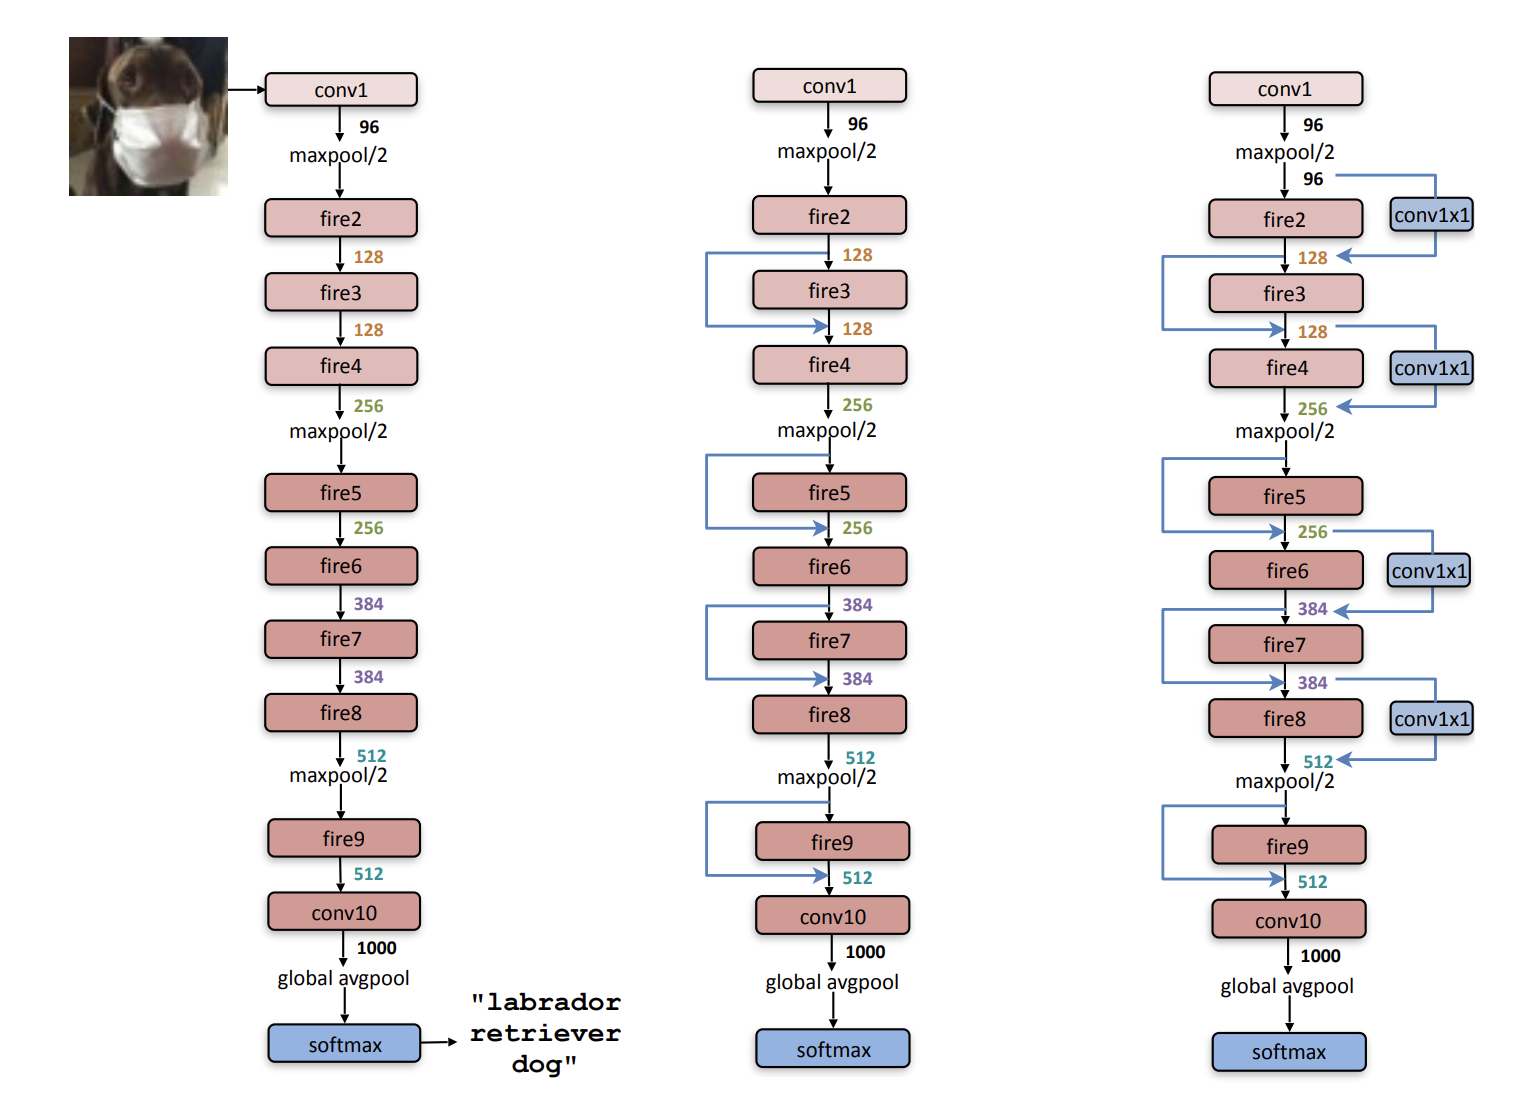
\includegraphics[scale = 0.2]{imagenes/squeezenet.png}
	\caption{Arquitectura de SqueezeNet}
\end{figure}


Esta red ha sido empleada en multitud de aplicaciones: detección de objetos en tiempo real, clasificación semántica, y modelos preliminares de conducción autónoma. Entre todas sus aplicaciones, podríamos destacar su utilización en imagen médica, concretamente MRI (Resonancias magnéticas). Ha permitido facilitar el diagnóstico de ciertas enfermedades y lesiones cerebrales en un espacio de memoria y recursos contenido.

Sin embargo, a pesar de las mejoras recibidas en sus versiones sucesivas, como los módulos Fire de doble nivel para reducir dimensionalidad, o la introducción de más reducciones mediante pooling, sacrifica resultados a nivel de accuracy respecto a la competencia, y no ha sido aplicada de forma firme y exitosa sobre imágenes de enfermedades cutáneas.



\subsection{MobileNet}
\label{cap:mobile}

MobileNet es el fruto del proyecto de investigación de Google Research para la implementación de redes convolucionales en dispositivos móviles. El objetivo era encontrar un modelo eficiente que pueda ser incluso utilizado en tareas de segmentación en tiempo real, pero reduciendo el número de parámetros del red así como el número de operaciones de producto necesarias, para poder ejecutarlas de forma nativa en dispositivos móviles como smartphones y tablets.\\

Esta arquitectura consta de 3 versiones diferentes, siendo cada una más sofisticada que la anterior. Disponemos de MobileNet V1, MobileNet V2 y MobileNetV3.

\subsubsection{MobileNet V1 (2017)}

La versión original de la arquitectura convolucional MobileNet  \cite{howard2017mobilenets} fue publicada en 2017. En esta publicación, se busca reducir el número de operaciones realizadas para conseguir un menor impacto de las operaciones en punto flotante sobre el rendimiento.\\
El punto clave de esta arquitectura reside en las llamadas "pointwise convolutions", haciendo uso del concepto de separabilidad, ampliamente estudiado desde el año 2012 por la literatura.

Las nuevas convoluciones descomponibles se pueden separar en dos pasos bien delimitados: la convolución en profundidad y la convolución puntual.

\begin{itemize}
    \item Las convoluciones en profundidad realizan el producto del filtro con el volumen de entrada capa a capa. Es decir, no se tiene en cuenta la dimensionalidad total de la imagen, sino que se realiza por cada nivel de profundidad el mismo producto. Esto reduce considerablemente el número de parámetros, ya que la dimensionalidad del problema es mucho menor.
    \item La segunda fase es la convolución puntual, cuyo objetivo no es más que acumular el producto de todas las capas calculadas independientemente mediante una simple combinación lineal, la cual es de coste computacional muy bajo.
    
    $$G_{k,l,m} =  \sum_{i,j}^{} K^{i,j,m} * F_{k+i-1,l+j-1,m}$$
\end{itemize}

Este producto es calculable eficientemente por las técnica de álgebra lineal GEMM, que permite aplicar propiedades de la suma y la multiplicación para el producto matricial de forma eficiente mediante Tensor cores.\\

En resumen, gracias a la separabilidad convolucional, se adquieren varias ventajas:
\begin{itemize}
    \item El número de productos se reduce considerablemente. Como se puede verificar en \cite{howard2017mobilenets} se traduce en una reducción de entre 8 y 9 veces el número de operaciones con respecto a las arquitectura tradicional de convolución
    \item Se reduce el espacio necesario en memoria.
    \item Se puede aprovechar el hardware específico.
    \item No se pierde precisión de cálculo gracias a que la separabilidad de convoluciones no afecta al resultado.
\end{itemize}

\begin{figure}[H]
	\label{depthwise}
	\centering
	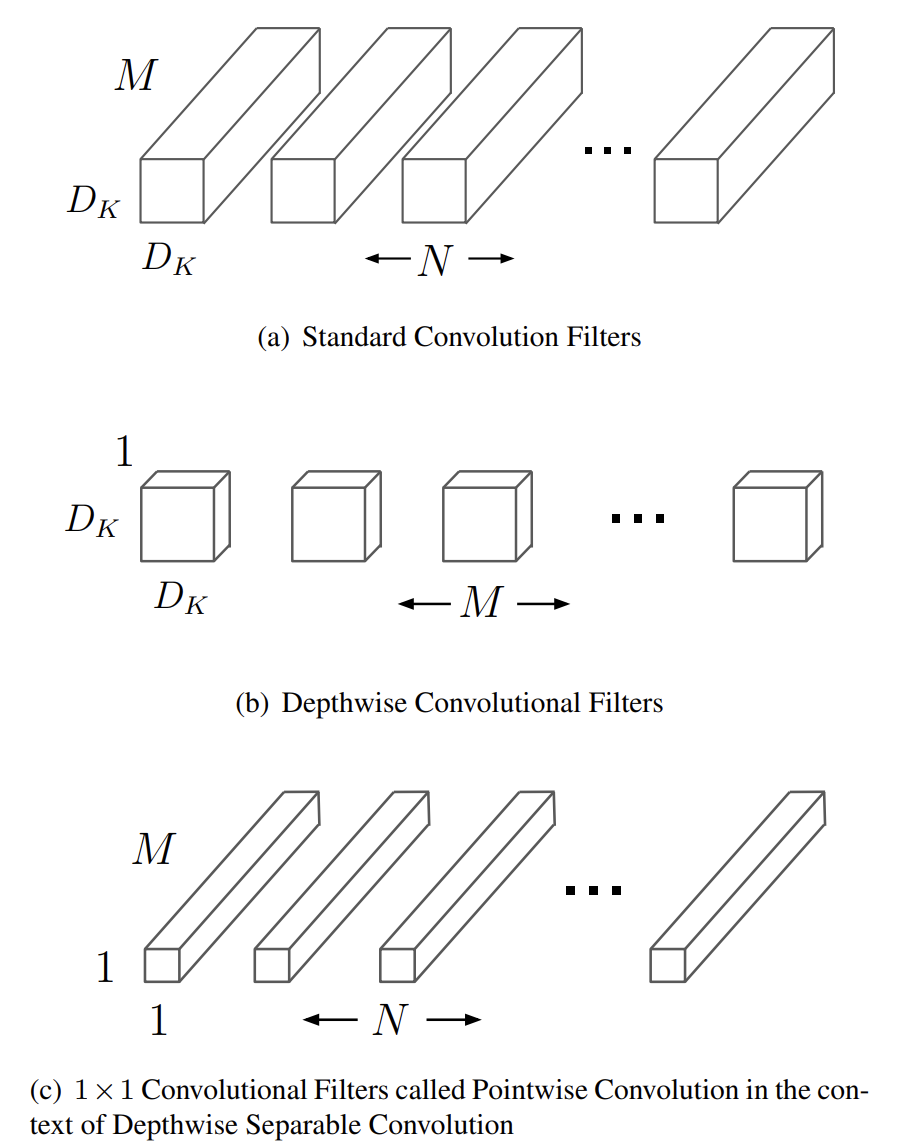
\includegraphics[scale = 0.225]{imagenes/depthwise.png}
	\caption{Producto depthwise}
\end{figure}

Adicionalmente, también incorporaron dos hiperparámetros: $\alpha$ y $\rho$. Estos parámetros controlan la anchura y la resolución de entrada, respectivamente.\\
El hiperparámetro $\alpha$ hace referencia a la anchura de cada capa convolucional que compone la red, adquiriendo un valor de 1 cuando la arquitectura no se ve reducida, y gradualmente podrá ser reducida en el intervalo (0,1]. Así se conseguirán modelos más simples en anchura para dispositivos con menores recursos.\\

En cuanto a $\rho$, este se encuentra implícito en la resolución de la imagen de entrada. Por defecto, la red acepta imágenes de hasta 224x224, pero en función de dicho valor $\rho$, podremos reducir su resolución también dentro del intervalo (0,1].\\

Ambos parámetros sacrificarán bondad y ajuste en los resultados a favor de una mayor eficiencia.

\subsubsection{MobileNet V2 (2018)}

Dos años más tarde de la publicación de MobileNets, da a luz su versión V2  \cite{sandler2019mobilenetv2}. Esta conserva los hiperparámetros  de la versión anterior, así como el producto punto a punto. Sin embargo, añade tres nuevas características, algunas de ellas no triviales y que requieren experimentación:
\begin{itemize}
    \item Se introduce el concepto de ``residuo invertido''. Ésta mejora reside en la utilización de los bloques residuales, propuesto por la arquitectura de ResNet. Su objetivo es evitar la degradación del gradiente, y que se frene el aprendizaje en modelos de gran profundidad. Normalmente, estas conexiones se realizan entre capas de gran profundidad, siendo las capas intermedias bloques estrechos. Sin embargo, en MobileNet V2, se propone la composición inversa, de forma que sean los bloques intermedios entre los residuales aquellos que poseen una mayor anchura, y así reducir el número de parámetros sin perder expresividad en el modelo \cite{invertedresidualsv2}.
    \begin{figure}[H]
    	\label{invert}
    	\centering
    	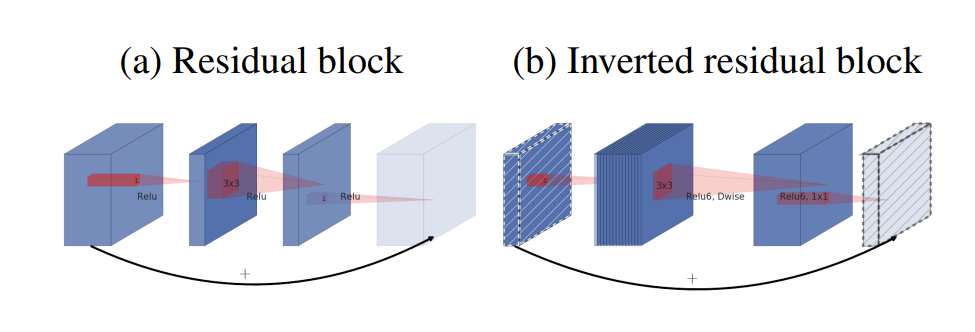
\includegraphics[scale = 0.3]{imagenes/invertedres.png}
    	\caption{Bloque residual invertido}
    \end{figure}
    
     \item En las capas donde el volumen de entrada es estrecho, al hacer uso de bloques residuales invertidos, la eliminación de la no linealidad aportada por ReLu favorece a la conservación de características y permite obtener mejores resultados de accuracy en tareas generales como clasificación en imagenet. Esto se debe a que al realizar los saltos entre bloques ``estrechos'' perdemos rendimiento de la red, y simplemente con eliminar la última transformación no lineal del bloque, contrarrestamos este problema.
    \item ReLu6. Se mantiene una versión modificada de la original función de activación. En lugar de utilizar la tradicional función ReLu entre 0 y 1, se extiende este intervalo hasta 6, permitiendo mantener la precisión en caso de utilizar coma fija, ya que se aseguran 3 dígitos de parte entera, y el resto queda destinado a la mantisa, que se almacena de forma precisa.
\end{itemize}

    \begin{figure}[H]
	\label{mv2}
	\centering
	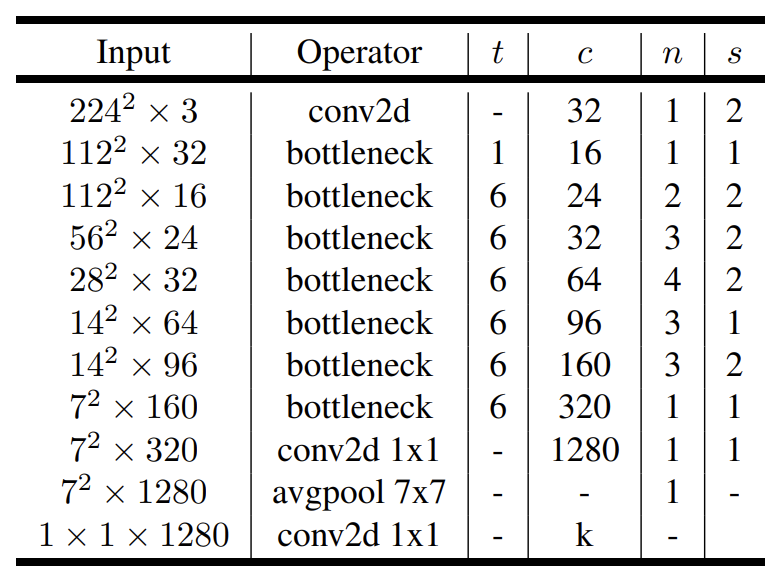
\includegraphics[scale = 0.25]{imagenes/mobilenetv2.png}
	\caption{Arquitectura de MobileNetV2}
\end{figure}

\subsubsection{MobileNet V3 (2019)}

En su tercera versión\cite{howard2019searching}, MobileNet incorpora métodos avanzados de diseños de redes basados en NetAdapt. Este algoritmo se basa en la transformación de modelos preentrenados para escritorio, y, en base a una serie de requisitos de potencia especificados, adapartar la arquitectura a una plataforma móvil perdiendo las mínimas capacidades posibles de la red original.  El modelo de partida empleado fue ajustado con precisión para mejorar latencias y uso de memoria, aplicando los siguientes conceptos:

\begin{itemize}
    \item Se añade la capa Squeeze-and-Excite, dentro de las conexiones residuales. Se trata de un mecanismo surgido en 2018 \cite{hu2019squeezeandexcitation}. Este estudio afirma que existen filtros de imagen con mayor importancia para el cómputo global que otros, como, por ejemplo, los bordes. Por tanto, les aporta un mayor ``peso'' durante el entrenamiento a dichos filtros haciendo uso de una serie de parámetros adicionales. Éstos añaden una carga computacional muy pequeña, por lo que se trata de una técnica eficaz. Para obtener los parámetros de relevancia, se dispone de dos módulos: squeeze, y excite. El módulo squeeze se encarga de representar cada filtro mediante un valor numérico, obtenido por average pooling de la imagen. Y por otro lado, el módulo excite se encarga de aprender los pesos que dar a cada uno de estos filtros o canales, haciendo uso de un MLP. El resultado final serán los pesos de cada canal en cuanto a su importancia, normalizados entre 0 y 1 por una función sigmoide.

    \item Se incluyeron nuevas capas al inicio y al final de la red de tipo residual invertidas.
\end{itemize}

    \begin{figure}[H]
	\label{mv2}
	\centering
	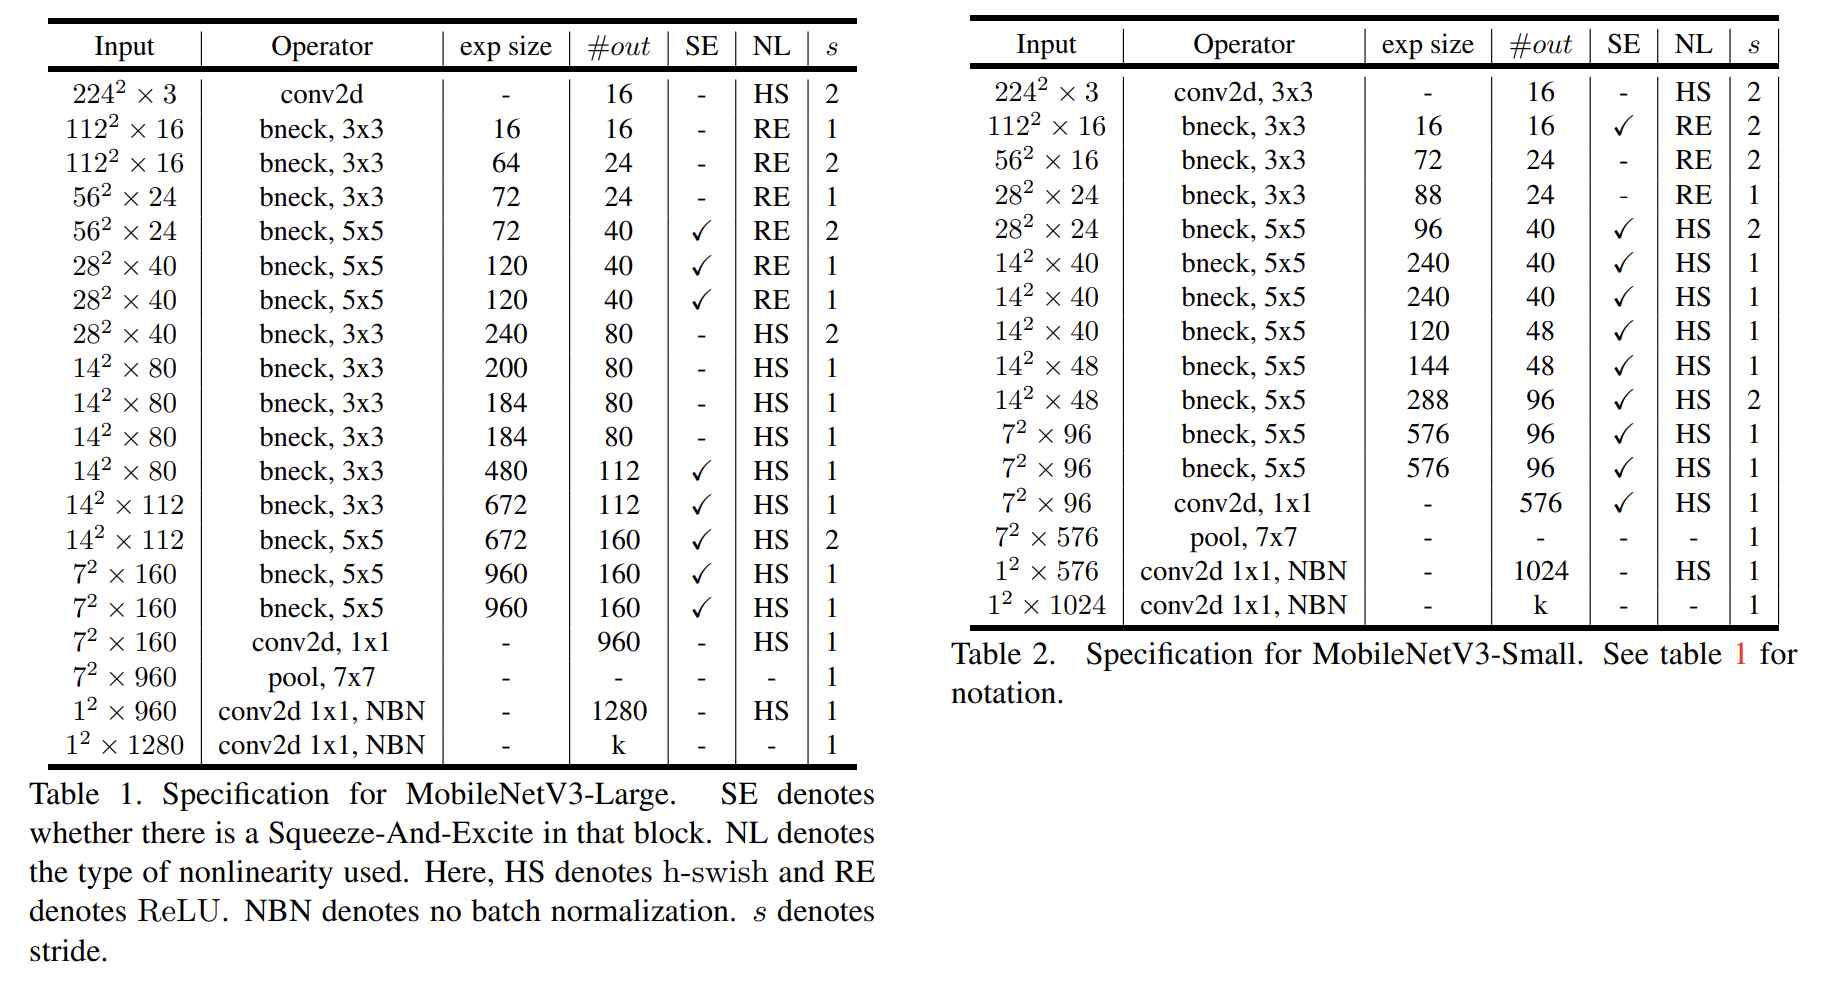
\includegraphics[scale = 0.85]{imagenes/mobilev3.png}
	\caption{Arquitectura de MobileNetV3}
\end{figure}

Debido a la gran complejidad adquirida por el modelo, los problemas de latencia y rendimiento en dispositivos de menor potencia, se opta por dividir la arquitectura en dos modelos parametrizables: MobileNet Small y Large. Mientras que la versión Large mejora los resultados de la versión 2 aumentando las prestaciones, el modelo Small otorga importancia sobre todo a la eficiencia y el uso de memoria, enfocado al hardware embebido o dispositivos de poca potencia.


\subsubsection{Aplicaciones en dermatología y cáncer de piel}

MobileNet, concretamente en su segunda versión, ha sido utilizado en la literatura para el diagnóstico de enfermedades de la piel. En \cite{Chaturvedi_2020}, es utilizado para realizar la clasificación de 7 enfermedades cutáneas extraídas del Humans against Machine, HAM10000 \cite{ham10000}, que podemos encontrar en ISIC archive \cite{isicarchive}, un repositorio web de acceso libre con enfermedades de la piel tanto beningnas como cancerosas. 

También se utilizó más recientemente para su implementación en dispositivos de IOT, \cite{mnetsqueeze}, donde se logra alcanzar el 99\% de accuracy en un pequeño conjunto extraido de ISIC, haciendo uso de la versión V3 junto a un algoritmo de Squeeze. Dicho algortimo se encarga de localizar la ubicación de los pelos y otros posibles artefactos para preprocesar la imagen y lograr una fotografía resultante libre de interferencias. 

Para ello, hace uso de un filtro black hat, que binariza la imagen y obtiene los píxeles objetivo de eliminar, que son sustituidos por los colores de los píxeles adyacentes, junto al uso del aumento de datos. Sin embargo, no queda especialmente claro la tasa de precisión del modelo para cada una de las enfermedades que se intentan diagnosticar.

\subsection{Shuffle Net}

Shuffle Net \cite{zhang2017shufflenet,shufflenetreview} surge con el objetivo ofrecer un modelo capaz de ofrecer un buen modelo con la mínima pérdida de rendimiento frente a modelos profundos. Es capaz de superar en resultados a la primera versión de MobileNet, logrando un error de aproximadamente tres puntos menos que MobileNet V1. Su mejor rendimiento se debe sobre todo al uso de Channel Shuffle para las convoluciones grupales, y creando una arquitectura basada en módulos shuffle.

La convolución en grupo mediante mezcla de canales (Channel Shuffle) surge tras el estudio del funcionamiento de las convoluciones grupales en 	AlexNet\cite{NIPS2012_c399862d} y ResNext. En ambos modelos, se uitilizan convoluciones grupales, donde cada canal de salida sólo se relaciona con los canales de entrada del que proviene. Esto podría debilitar la relación entre cada canal, y debilitar los resultados; para evitarlo, y no poner en riesgo el rendimiento con demasiadas convoluciones 1x1 para relacionarlos, se hace uso del mezclado de canales; es decir, es como si permitiésemos que cada grupo convolucional pudiera obtener información de otros grupos adyacentes, para así mejorar la relación entre ellos.

Para evitar un sistema complejo a la hora de representar dichas interconexiones, es como surge el channel shuffle \ref{shufflechannels}: se mezclan los canales de forma que los grupos ya no quedan aislados con sus respectivas entradas y salidas.

    \begin{figure}[H]

	\centering
	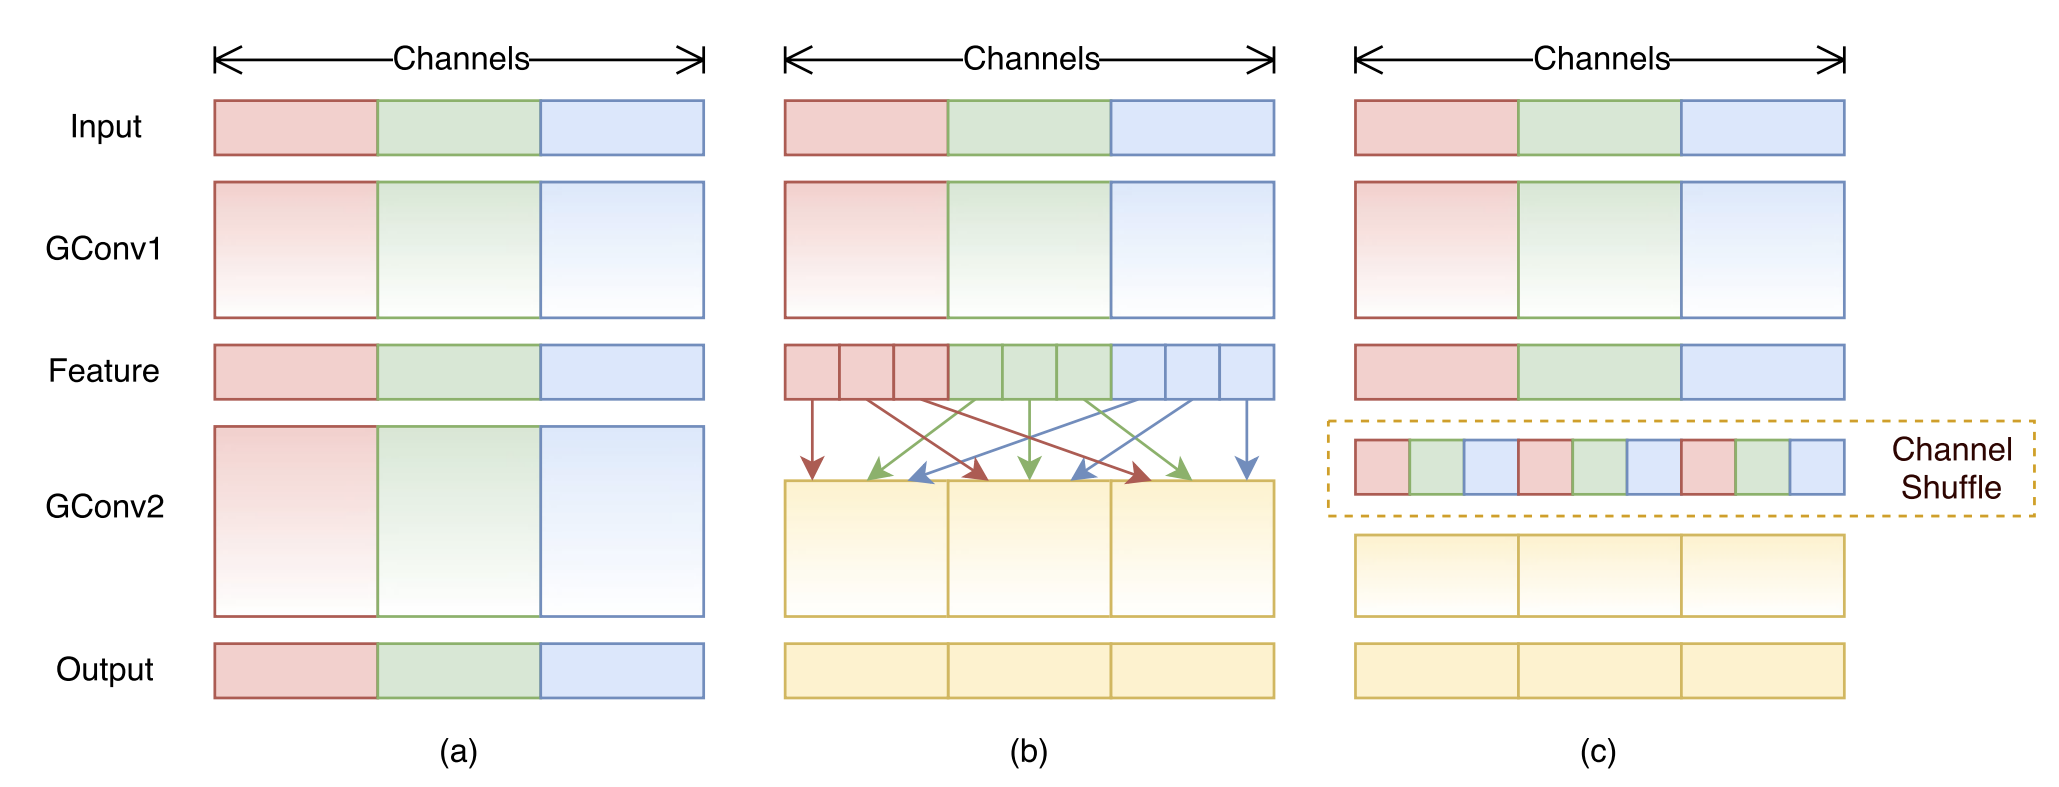
\includegraphics[scale = 0.2]{imagenes/shufflechannels.png}
	\caption{Channel Shuffle de ShuffleNet}
	\label{shufflechannels}
\end{figure}

Esta técnica se aplicará sobre la primera y última convolución 1x1 realizada sobre los bloques residuales de la red, que siguen una estructura parecida a la que adoptaría MobileNetV2 posteriormente. Mediante esta propuesta, podemos además aplicar una mayor capacidad de procesamiento en anchura añadiendo stride, y aplicando average pooling. El resultado, es conseguir modelos más anchos en procesamiento que no impacten negativamente en el rendimiento de los dispositivos con menor capacidad. En la figura \ref{arquitecturashuffle} , podemos apreciar la arquitectura de la red, cuyos filtros pueden ser escalados mediante el parámetro s, aunque teniendo en cuenta una penalización en la complejidad, equivalente a $s^2$ sobre Shuffle Net base, equivalente a $s=1$

\begin{figure}[H]

		\centering
		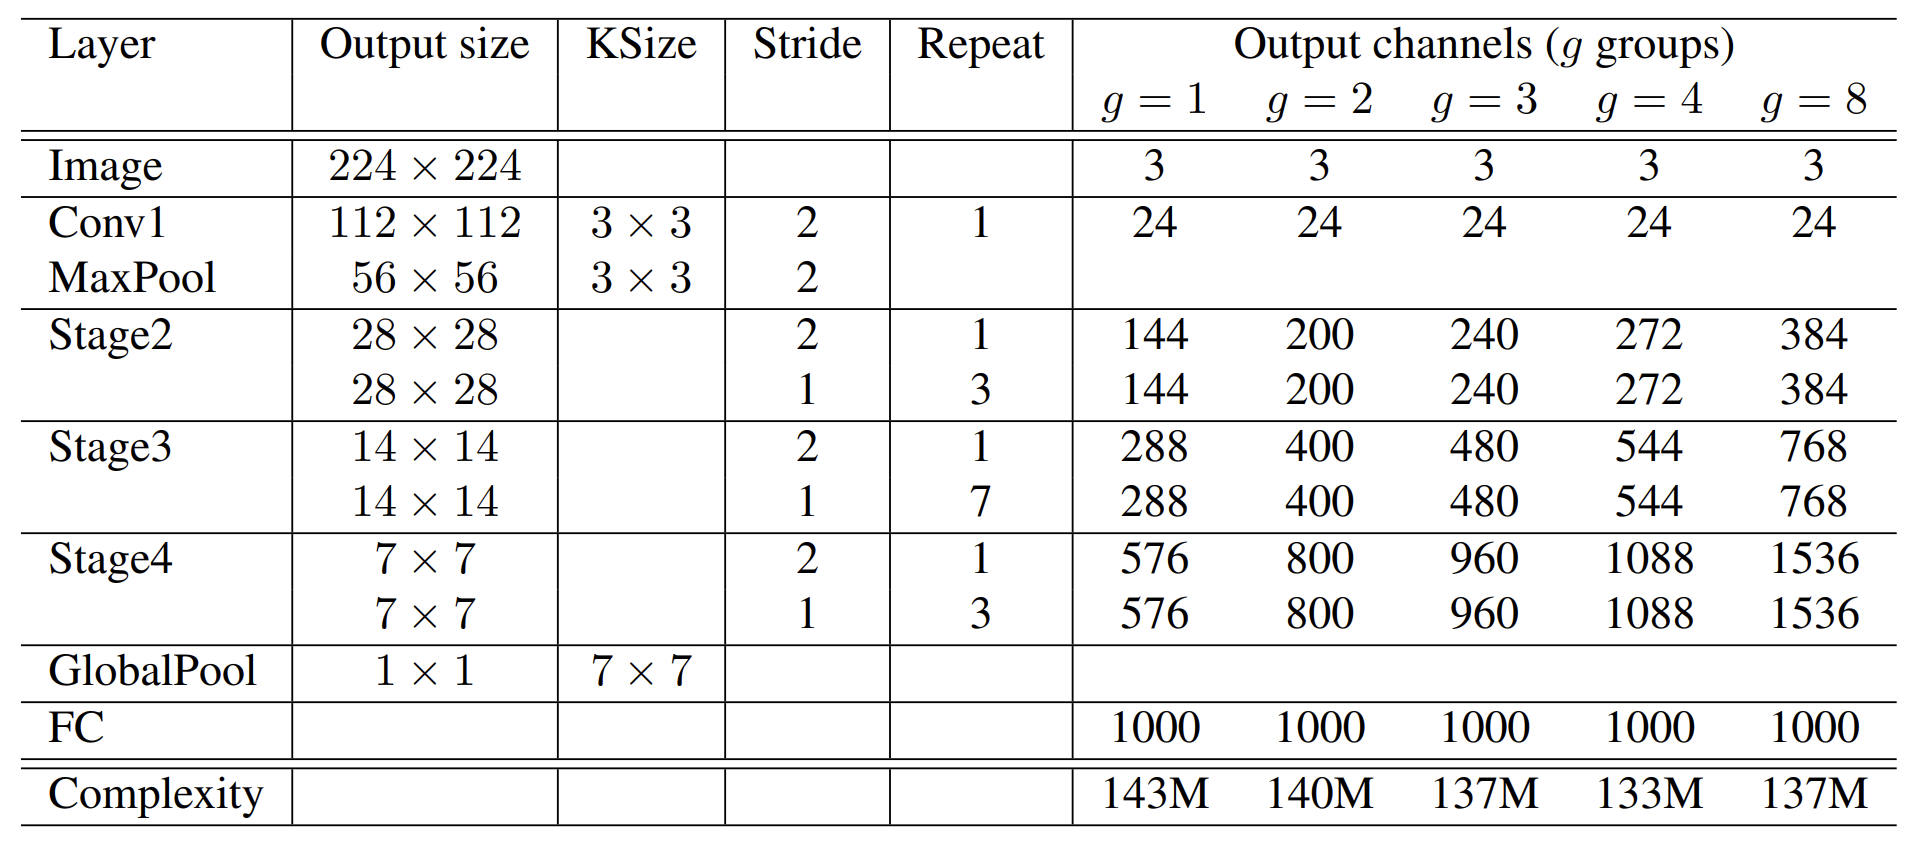
\includegraphics[scale = 0.2]{imagenes/arquitecturashuffle.png}
		\caption{Arquitectura de ShuffleNet}
		\label{arquitecturashuffle}
	\end{figure}

Sus aplicaciones han sido variadas, pero en lo que respecta a la detección de lesiones cutáneas, la cercana salida de MobileNet V2 y su mejor rendimiento provocó que ShuffleNet quedase relegada a un segundo plano, y no fuese muy utilizada para este fin. Podemos encontrar algunos trabajos \cite{shuffleapp} donde podemos observar una comparativa de este modelo frente a la completitud de los modelos del estado del arte de 2022, y podemos confirmar que  MobileNetV2 es capaz de superar su rendimiento en la mayoría de pruebas, siendo estas comparaciones en cuanto a tiempo de entrenamiento, precisión, accuracy y tamaño del conjunto de entrenamiento. Sólo consigue superar a MobileNetV2 en tiempo de entrenamiento, donde es aproximadamente 900 más rápida, pero ofrece peores resultados en promedio.

\subsection{EfficientNet}
\label{efnetcap}

EfficientNet \cite{Chaturvedi_2020} es un conjunto de arquitecturas de redes creadas por el departamento de investigación de Google con el fin de conseguir una familia de modelos variada que fuese capaz de adaptarse fácilmente mediante parámetros a diferentes conjuntos de imágenes, y a requisitos de hardware más o menos limitados. 

Parte de que una red convolucional sigue el siguiente esquema:
$$\mathcal{N}=\odot_{i=1...s} F_i^{L_i}(X_{(H_i, W_i,L_i)})$$


Donde se denota que la capa $F_i$ es repetida $L_i$ veces la etapa i de la red, y la dimensionalidad de la capa queda representada con ${( W_i,L_i)}$.  Fijando $F_i$, efficient net intenta dar versatilidad a sus modelos variando las dimensiones restantes, Li, Ci, Hi, Wi mediante el uso de 3 constantes de escalabilidad \ref{fig:paramsefnet}:

\begin{itemize}
	 \item  Profundidad, Depth (d):  Aumentar la profundidad es la tendencia habitual presente en las redes convolucionales. Pero llegar a un equilibrio es crítico, ya que aumentar demasiado la profundidad sin modificar otros parámetros puede ocasionar pérdidades rendimiento por el desvanecimiento del gradiente  a menor profundidad. 
	\item Anchura, Width (w): Aumentar la anchura suele ser beneficioso para modelos de pocos recursos donde el aumento de profundidad supone un gran aumento de la carga computacional. Permite conseguir mayor cantidad de características de grado fino, pero si la red es demasiado poco profunda, el modelo careceré de características de alto grado que permitan aprender patrones generales.
	\item Resolución, (r): al emplear tamaños de entrada mayores, damos opciones a obtener una mayor cantidad de características de grado fino, pero un exceso de resolución puede provocar grandes tiempos de ejecución y puede ser contraproducente, al reducirse la ganancia con tamaños demasiados grandes.
\end{itemize}

\begin{figure}[H]
	\centering
	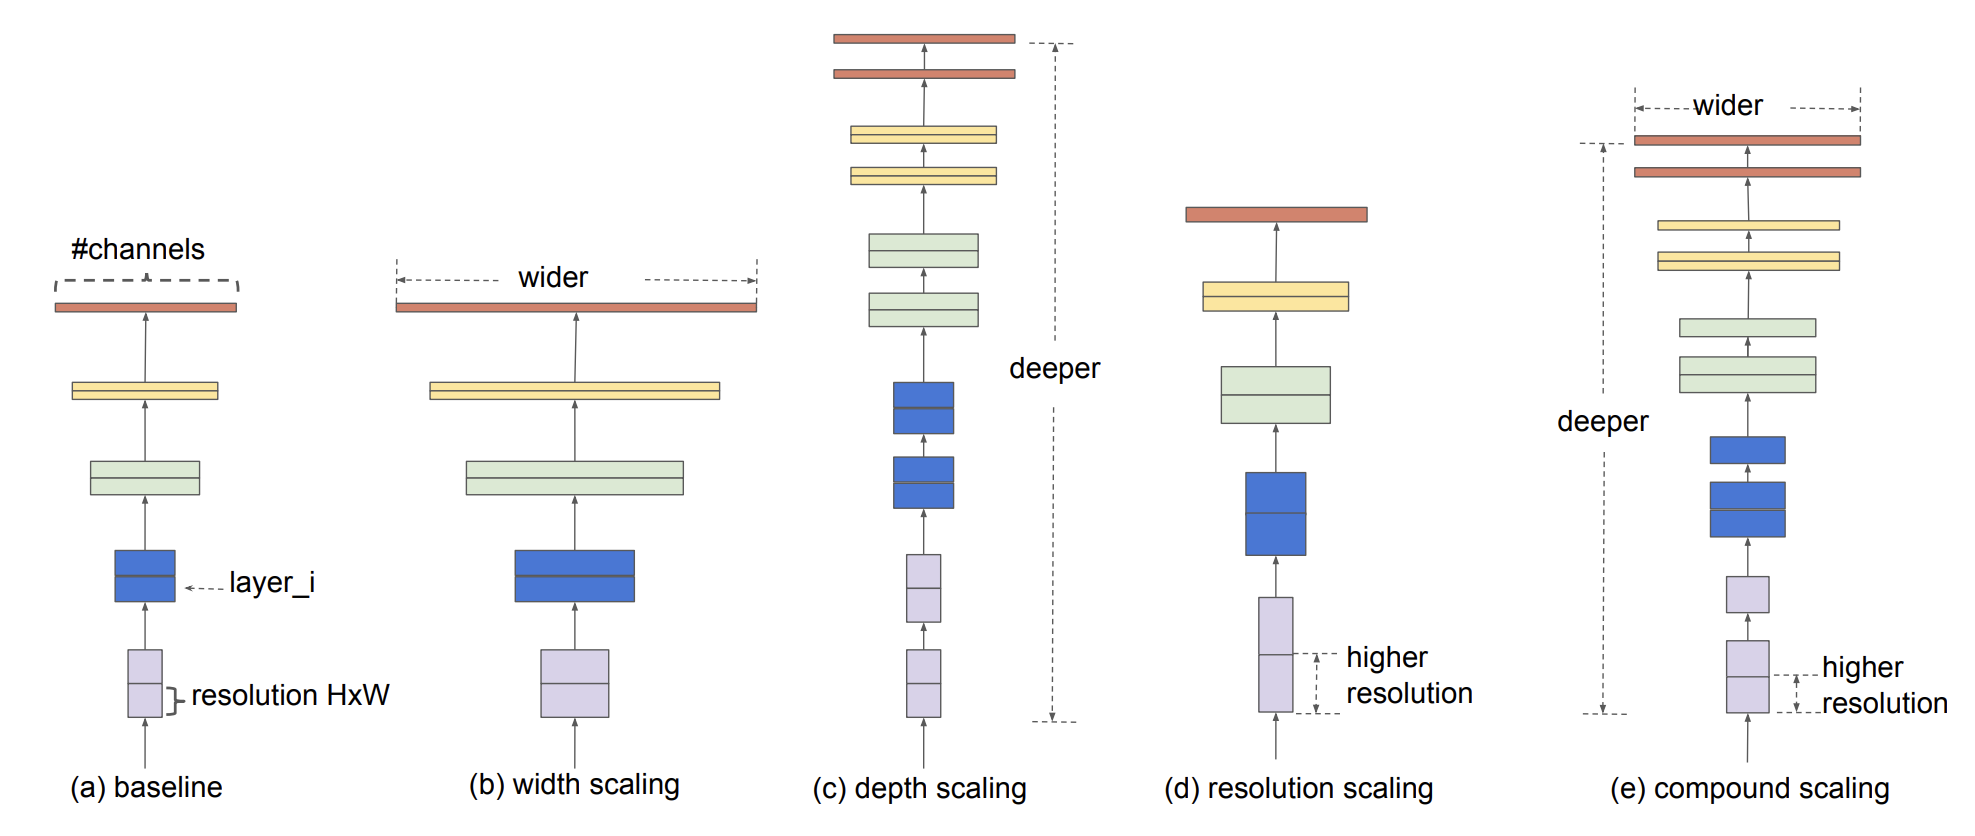
\includegraphics[scale = 0.2]{imagenes/efnet_scale.png}
	\caption{Parámetros de EfficientNet}
	\label{fig:paramsefnet}
\end{figure}


Experimentalmente, estos parámetros pueden ser ajustados, y dan lugar a una serie de modelos distinto: los conocidos EfficientNetB0 - B7, denotando el valor numérico la profundidad y complejidad del modelo, siendo esta mayor a mayor valor del índice.	 Cada una de ellas fue ajustada utilizando una profundidad concreta, y puede ser posteriormente ajustada con el resto de parámetros libres no fijados a las características del conjunto de entrada.

En smartphones de alta gama, los modelos B0 a B4 pueden ser ejecutados con un rendimiento aceptable para aquellas aplicaciones que no requieran un alto tiempo de respuesta, pero si necesitan dar al usuario una respuesta aceptable. Para modelos de mayor complejidad computacional, se usan las variantes lite, que estudiaremos más adelante.


\subsubsection{Aplicaciones en dermatología y cáncer de piel}

En el problema que nos concierne, esta arquitectura ha conseguido grandes resultados en el dataset del ISIC abierto al público como competición en la plataforma Kaggle, habiendo sido utilizado como parte de un ensemble de modelos, o bien como modelo único entrenado en el top 3 de ganadores de la competición. En el caso de la segunda mejor solución clasificada \cite{2ndISIC}, se menciona la utilización de EfficientNet-B6, con tamaño de entrada de 512x512, y un tamaño de batch de 64, obteniendo 0.9485 de accuracy como resultado final a la hora de emplear los datasets ISIC 2019 y 2020\\ En la primera solución, es usada en conjunto a Resnet50, y una red especializada en los metadatos de la imagen, y todos los modelos juntos someten su resultado a votación \cite{1stISIC}.

Ambos resultados han sido evaluados con computadores de alta gama, haciendo uso de múltiples tarjetas gráficas para el entreanmiento y la inferencia. Este proceso es demasiado pesado para un dispositivo móvil, por lo que de cara a este trabajo, se buscarán alternativas capaces de ahorrar en espacio y potencia como concepto de cuantización.

 \section{Cuantización de modelos}
\label{cap:cuantización}
Las arquitecturas y soluciones propuestas por la literatura que han sido analizadas en los apartados anteriores proponen métodos que ofrecen buenos resultados. Sin embargo, existe un problema: todas ellas han sido entrenadas con un computador cuya capacidad de cálculo supera incluso las características de un ordenador doméstico promedio, como en \cite{2ndISIC}, donde se emplean 4  GPU Nvidia Quadro RTX 6000 24GB. Aunque su utilización engloba sobre todo el proceso de entrenamiento, la inferencia de estos modelos también sigue siendo extremadamente costosa para un dispositivo móvil, y este proceso también es realizado a través del computador.

Esto resume a que el teléfono simplemente adquiere el papel de cliente dentro de una arquitectura cliente-servidor, donde el dispositivo host de todo el procesamiento de la imagen y de su clasificación es un ordenador de gran potencia de cálculo, y el teléfono movil únicamente debe compartir con este la imagen que desea examinar. Pero esto supone una gran desventaja: en ausencia de conexión de red, o interrupción del servicio por parte del servidor, el usuario no sería capaz de emplear la aplicación para el diagnóstico. La dificultad e interés de este proyecto se ve reforzado por este argumento, y resulta ahora de interés la posibilidad de realizar la inferencia en el teléfono, a pesar de que el entrenamiento sea realizado en un ordenador.

Existe una técnica que nos permitirá obtener un modelo optimizado a partir de uno entrenado de forma tradicional: la cuantización.

\subsection{Características}

La cuantización de modelos se centra en la simplificación y optimización de un modelo preentrenado por un computador, reduciendo algunas de sus características buscando un impacto mínimo sobre los resultados obtenidos, pero reduciendo de forma considerable el tiempo de inferencia para dispositivos de baja potencia. Aunque existen mecanismos de poda, donde la arquitectura del modelo se ve simplificada de forma directa, el método que evaluaremos será la cuantización de modelos basada en la reducción de la precisión numérica, es decir, una disminución en la profundidad en bits de la variable flotante.

Este concepto ya fue brevemente mencionado durante el desglose de características de MobileNet V3 \cite{howard2019searching}. En la arquitectura AMD64, el almacenado de variables en coma flotante emplea una precisión de 32 bits. Por tanto, al realizar operaciones de cualquier tipo, las 32 posiciones del nuevo número han de ser actualizadas al valor resultado. El tiempo empleado en realizar dicha operación en cada dígito de este número puede parecer despreciable, pero, cuando el conteo de operaciones alcanza los miles de millones, supone una diferencia significativa en el rendimiento. 

En dispositivos de baja potencia, esta precisión suele verse reducida a 8 bits, de forma que reducimos la longitud del máximo número almacenable en 4 veces menos, y reducimos también así el tiempo por operación.

Este mecanismo es empleado tanto por los frameworks de trabajo habituales para aprendizaje mediante redes convolucionales, como Pytorch y TensorFlow, y por los propios fabricantes de teléfonos móviles de forma nativa. Es el caso de Qualcomm, conocido por su gama de procesadores Snapdragon. Esta empresa realizó un estudio del impacto de la cuantización en los modelos \cite{kuzmin2024fp8} usando flotantes de 8 bits del precisión. Demuestran que el uso de números flotantes de 8bits en lugar de enteros con exponenciación para desplazar el punto ofrece un mayor rendimiento. Las consideraciones a la hora de defender la utilidad de la cuantización son las siguientes:

\begin{itemize}
	\item La operación más costosa realizada durante la inferencia es el producto de matrices. Para simplificar la complejidad de la operación, normalmente se suelen emplear matrices de números enteros reescalados a un nuevo intervalo de valores. Esto es, se aplica una transformación de rangos, donde una matriz $\mathbb{R}^{m x n}$ se cuantiza a una matriz $X^{(int)}$ asociado a un valor de reescalado s: $X^{(int)}=clip([\frac{X}{s}],x_{min},x_{max})$, donde el producto pasa a ser el valor redondeado más cercano al número tras aplicar la transformación de rango mediante escala, y la operación de clip asegura que el número es representable dentro de los valores establecidos para el extremo. Esto proporciona una simplificación contra la habitual notación IEEE-754 de 32-bit, FP32, donde se usa un bit de signo, 23
	de mantisa, y 8 bits de exponente.
	\item  La utilización de FP8 puede ser beneficiosa al ser capaz de encontrar un término medio entre la precisión y variabilidad de rango numérica del resultado, como se puede ver en \cite{kuzmin2024fp8}. Los resultados empíricos muestran que tras un ajuste entre el número de bits de mantisa y exponente, se logra un equilibrio adecuado usando valores cercanos a 3 bits de mantisa y 4 de exponente, y en caso de post training quantization, 5 de mantisa y 2 de exponente, en caso de que el aprendizaje se realice de forma lenta.
	\item Para mejorar estos resultados, se puede usar la técnica Quantization Aware Training (QAT), o entrenamiento preparado para cuantización, donde el objetivo es facilitar el paso a FP8 desde el proceso de entrenamiento teniendo en cuenta los rangos de valores adoptados durante el entrenamiento, como por ejemplo, controlando el diferencial mínimo que puede tomar el algoritmo de optimización. Esta operación muestra mejor resultado sobre valores enteros, pero también es capaz de mejorar los resultados obtenidos por PF8.
\end{itemize}

En los frameworks Pytorch y TensorFlow, podemos encontar estas optimizaciones en sus funcionalidades relacionadas con la optimización de modelos en post entrenamiento, con las dependencias de Pytorch Mobile y TensorFlow lite, respectivamente. Ambas aplican cuantización numérica de los tensores, y en caso de tratarse de modelos tradicionales de la literatura, existen arquitecturas simplificadas de forma profunda, con redes como EfficientNet o ResNet, que cuentan con variantes lite.

\subsection{Modelos cuantizados}

El framwork de TensorFlow lite contiene dos de los modelos más utilizados en la literatura en sus variantes lite: EfficientNet Lite y ResNetV2. Ambos han recibido un tratamiento de simplificación, que pasa por el uso de INT8 como modelo de representación numérica y la simplificación de la arquitectura, retirando algunas de las capas más resentidas en el proceso de optimización. En el caso de EfficientNet Lite, podemos encontrar un descripción detallada sobre aquellos cambios realizados para la mejora de rendimiento \cite{eflite2}:

\begin{itemize}
	\item Se hace uso de cuantización post entrenamiento mediante el algoritmo de cuantización empleado por Tensorflow lite. Esta cuantización se hace de forma dinámica, dependiendo del hardware en el que se ejecuta el modelo. Puede realizarse una cuantización de rango dinámico, donde el factor de escalado puede aplicarse de forma distinta dependiendo de la capa en la que se realice la operación; cuantización de enteros, para los dispositivos menos potentes; y 	por último, cuantización de FP16, de forma que se logra un término medio entre ambas soluciones, y se puede emplear en dispositivos con GPU de potencia considerable. Por defecto, es la opción de rango variable la utilizada.
	\item Se eliminan algunos módulos Squeeze and Excite presentes en capas intermedias, debido a su coste e imprecisión para dispositivos que no soportan gran precisión numérica.
	\item Las funciones de activación se reemplazan con RELU6, al igual que se realizó en MobileNetV3 \cite {howard2019searching} 
\end{itemize}

\begin{figure}[H]

	\centering
	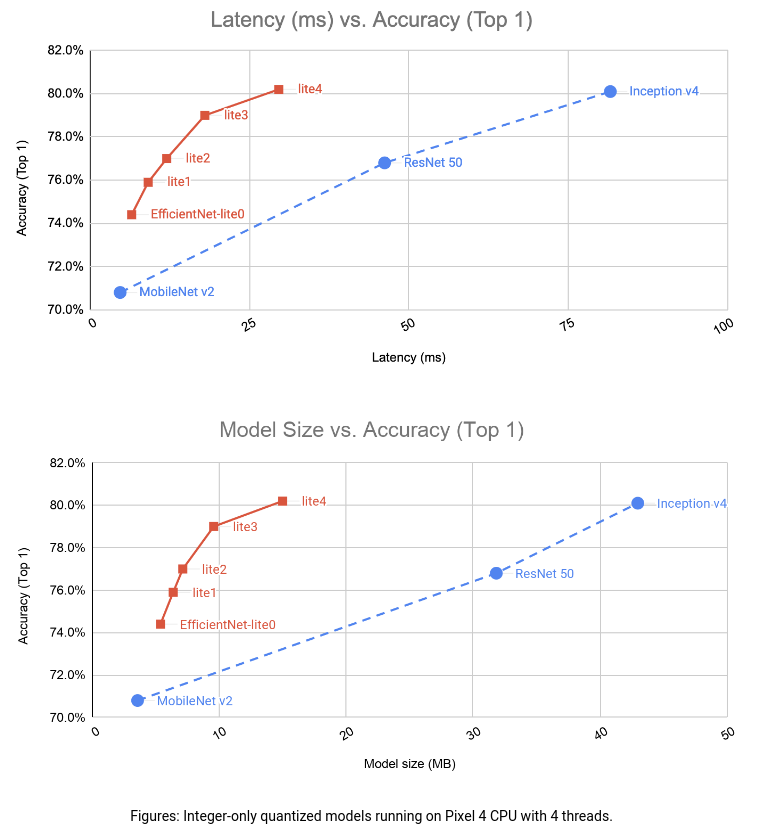
\includegraphics[scale = 0.325]{imagenes/eflite.png}
	\caption{Optimización de EfficientNet Lite}
		\label{eflite}
\end{figure}

Este procedimiento variable, con múltiples posibles combinaciones, se realiza debido a la gran variedad del mercado actual. Existe una gran diversidad de  dispositivos: conviven dispositivos de bajo consumo con escasa potencia gráfica, así como terminales especializados con unidades de TPU para acelerar el cálculo neuronal. Y, de esta forma, con optimizaciones modulares, podemos priorizar la eficiencia en dispositivos con poca capacidad de cálculo , y aumentar la precisión en aquellos que pueden ejecutarlos. En el dispositivo de ejemplo, un Google Pixel 4, se consigue un tiempo medio de inferencia de 30 ms, una mejora de casi el 60\% sobre ResNet50.

\subsection{Conclusión de los modelos cuantizados}

A la vista de los resultados, los modelos cuantizados pueden suponer una ventaja; obtenemos resultados cercanos a los modelos complejos del estado del arte, con una pequeña penalización ganada en forma de rendimiento, y que la ejecución ofrezca tiempos de respuesta razonables. Además, este tipo de transformaciones no se han empleado para el reconocimiento y detección de enfermedades de la piel, y abren una nueva linea de investigación en la que obtener resultados.

Como puntos en contra, debemos tener en cuenta que la penalización obtenida al entrenar este tipo de modelos no es siempre la misma; dependiendo del problema a clasificar, y del modelo seleccionado, la penalización de la cuantización puede ser o no más marcada; para ello, es necesario obtener empiricamente resultados que nos permitan conocer el tipo adecuado para nuestro problema. Este conflicto para encontrar el equilibrio ya fue detectado por los desarrolladores de Google en EfficientNet Lite \cite{eflite,eflite2}, donde inicialmente, sus pruebas en ImageNet arrojaron resultados pésimos al obtener un 46\% de accuracy en clasificación TOP1 a diferencia del 75.1\% obtenido con FP32. Pero, tras ajustar el rango de amplitud de los enteros utilizados para cuantización, se consiguió una ganancia de 1.85x sobre el modelo original con tan solo un 0.7\% de pérdida en los resultados.

\begin{figure}[H]

	\centering
	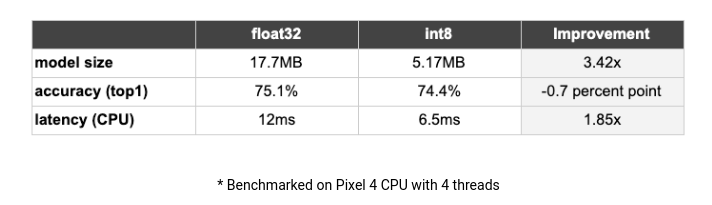
\includegraphics[scale = 0.35]{imagenes/gananciacuant.png}
	\caption{Ganancia de la cuantización en EfficientNet}
	\label{gananciacuant}
\end{figure}

Como aspecto negativo, aunque la varianza de los resultados pueda verse paliada mediante la selección de la cuantización más adecuada, aún existen riesgos de resultados inesperados. Con este mismo modelo, por ejemplo, se han alcanzado resultados inesperados, como que los modelos de menor tamaño (B0,B1,B2) poseen un mejor desempeño que B3 y B4 en datasets de propósito general, como podemos observar en el artículo de Agarwal  \cite{efliteworse}, pero esto puede deberse por la necesidad de una mayor cantidad de datos para realizar el entrenamiento.

Dado a los buenos resultados en general, la cuantización será la senda seguida por este TFG a la hora de optimizar los modelos de escritorio en post entrenamiento.


\newpage
\section{Conjuntos de datos disponibles}

La obtención de datos para el proceso de aprendizaje automático es una fase crucial para la obtención de un modelo correctamente entrenado y que proporcione resultados de calidad. Esta fase es un factor común en todos los problemas de aprendizaje, ya que a mayor diversidad y cantidad de datos, más cercana será la muestra de la que disponemos y, por ende, más cercanos serán los resultados al diagnóstico real. Múltiples puntos de vista, tonos de iluminación, y otro tiempo de variantes pueden ser  beneficiosas.

Para el diagnóstico del cáncer de piel, este proceso es igualmente importante. La piel es el órgano más extenso del cuerpo humano, y debido a que es el área de mayor esposición diaria a los elementos, presenta una gran variedad en cuanto pigmentación, porosidad, y otros elementos influyentes como el envejecimiento o el daño provocado sobre ella. Esto provoca que el diagnóstico de las lesione sea complejo, pues existen tanto lesiones benignas como malignas de gran similaridad. Además, cada localización geográfica del mundo posee diferentes tonos de piel., claros y más oscuros. La inexistencia de un tipo de piel o de lesión en el conjunto de entrenamiento podrían provocar resultados sesgados indeseados durante la predicción de la imagen tomada.

En la red, podemos encontrar varios reposotorios de imágenes cutáneas de acceso público,  que permiten su utilización de forma abierta con fines académicos para el desarollo de modelos de inteligencia artificial. Sin embargo, no todos ellos son indicados para su uso, ya que el control realizado sobre el diagnóstico y la certeza de los mismos puede ser verificada en mayor o menor medida, y necesitamos que estos sean los más fiables posibles. Es crítico desarrollar un plan de búsqueda que nos facilite la decisión de tomar o desechar un conjunto de datos que encontremos.

Para facilitar este proceso, podemos apoyarnos en diferentes artículos recientes donde se analizan los conjuntos de datos públicamente accesibles en la actualidad, y conocer la calidad de la imagen, el porcentaje de fiabilidad del etiquetado y el balance de clases. Destacamos el estudio realizado por M. Goyal et Al.  \cite{goyal2020artificial}, o el reciente artículo de  Sana Nazari y Rafael García \cite{life13112123}, donde se analiza la disponibilidad de los datasets a fecha de 2023.

Basado en sus estudios y recomendaciones acerca de los conjuntos de datos disponibles, he elaborado un diagrama de flujo a seguir para evaluar qué conjuntos decartar y cuales anotar para su uso en el entrenamiento:

\begin{figure}[H]
	\centering
	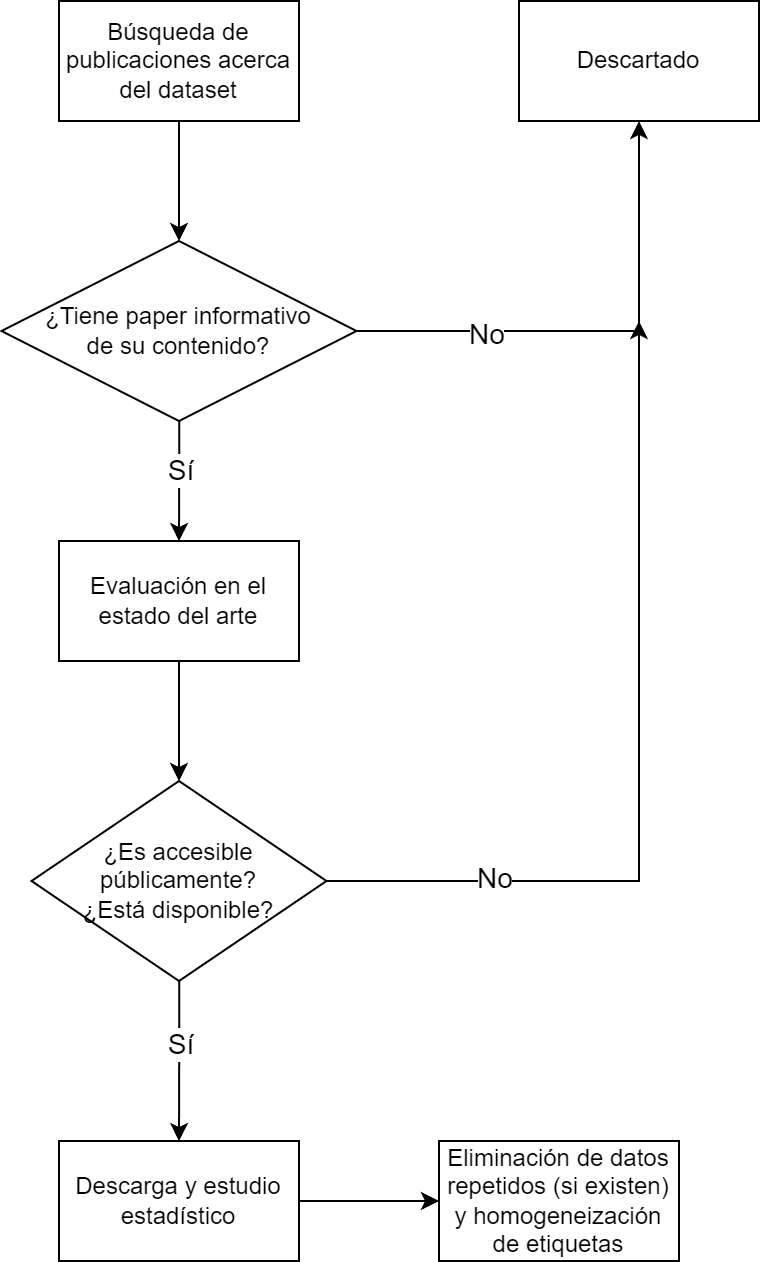
\includegraphics[scale=0.7]{imagenes/DiagramaBusqueda.png}
	\caption{Proceso de búsqueda seguido}
\end{figure}

Siguiendo dicho procedimiento, se han encontrado 6 datasets diferentes, cuyo origen son instituciones públicas que han cedido datos con fines académicos y de investigación.\\

Un factor determinante para la elección de estos conjuntos es la diversidad. Es indispensable, para este proyecto, encontrar datos lo suficientemente variados como para distinguir lesiones cancerígenas y no cancerígenas, y disponer de diferentes tonos de piel para entrenar. Aunque los tonos de piel más oscuras sufren lesiones de tipo cancerígeno en menor proporción gracias a su protección natural, también pueden sufrir este tipo de patologías, y es clave ser capaces de detectarlas en cualquier posible paciente.

\subsection{International Skin Imaging Collaboration​ (ISIC)}
El repositorio ISIC (International Skin Imaging Collaboration \cite{isicarchive}), es un repositorio en línea sin ánimo de lucro que recoge datos procedentes de diferentes instituciones públicas para elaborar un atlas online donde obtener datos para mejorar el diagnóstico de enfermedades cutánea y ofrecer un conjunto de imágenes accesible para la Inteligencia aritificial.

Dispone de un buscador de imágenes en el que se pueden filtrar las enfermedades de las que se deseen obtener imágenes o metadatos para su estudio. En su mayoría, las imágenes que podemos encontrar son de enfermedades benignas, pero la web hace especial énfasis en disponer de imágenes demoscópicas de lesiones principalmente cancerosas.  En la literatura, se trata de uno de los conjuntos de datos más citados, debido a su utilización anual durante los años 2016-2020 para la realización de un reto virtual de Machine Learning descrito. 

El objetivo era modificada cada año, pero este oscilaba entre la identificación de melanomas frente a lesiones no cancerosas, como se propone en el ISIC Challenge-2020 \cite{Rotemberg_2021}, o bien, identificar diferentes subtipos de lesiones cancerosas frente a lesiones benignas en la competición ISIC Challenge 2019, \cite{ham10000,codella2018skin,combalia2019bcn20000}, cuyo propósitos se acerca más al objetivo de este trabajo.

En el estado del arte, destacan las soluciones que hacen uso de métodos de Deep Learning, como el planteado por Ian Pan \cite{2ndISIC}] o el ya analizado anteriormente ganador del año 2020 \cite{1stISIC}, que realiza un enfoque híbrido por votación entre modelos que hacen uso de redes convolucionales para la clasificación de los datos de tipo imagen, y clasificación mediante Machine Learning para los metadatos.

Debido a que cada uno de estos subconjuntos de datos anuales eran escasos para modelos profundos, normalmente se ha recurrido a la reutilización de los conjuntos anteriores para enriquecer el conjunto de entrenamiento.  Se trata de una técnica que permite obtener buenos resultados ya que, a mayor conjunto de entrenamiento, más cercana será la muestra a la población real.  Hay que prestar especial atención a la repetición de datos, ya que la aparición duplicada de imágenes podría provocar un sobreaprendizaje sobre dicho ejemplar, además de posibles fugas de información entre entrenamiento, validación y test, al poder existir imágenes exactamante iguales entre ellos.

\subsubsection{Fusión y deduplicado}

Podemos encontrar una análisis del procedimiento de unión de los subconjuntos en  \cite{CASSIDY2022102305}. En este artículo, se realiza una análisis exhaustivo de los datos disponibles, cubriendo aspectos como métodos de deduplicado de imágenes, y una clasificación de posibles modelos a aplicar.

Si desglosamos el conjunto de datasets disponibles, nos encontramos con 5 conjuntos:
\begin{table}[H]
	\centering
	\begin{tabular}{|l|l|l|l|l|}
		\hline
		\textbf{Challenge Dataset Year} & \textbf{Train} & \textbf{Test} & \textbf{Total} & \textbf{Tipo de problema } \\ \hline
		ISIC 2016 & 900 & 379 & 1279 & Clas. binaria  \\ \hline
		ISIC 2017 & 2000 & 600 & 2600 & Clas. Multiclase  \\ \hline
		ISIC 2018 & 10015 & 1512 & 11527 & Clas. Multiclase  \\ \hline
		ISIC 2019 & 25331 & 8238 & 33569 & Clas. Multiclase  \\ \hline
		ISIC 2020 & 33126 & 10982 & 44108 & Clas. Binaria  \\ \hline
	\end{tabular}
\end{table}

\begin{itemize}
	
	\item ISIC 2016 \cite{gutman2016skin}:  Es el dataset de menor tamaño de todos los propuestos. Hace distinción únicamente de los casos malignos y benignos. Contiene imágenes dermoscópicas anotadas con información acerca de la localización de la mancha, y la edad del paciente. Contiene información adicional para la segmentación de la mancha pigmentada de interés (máscaras).
	\item ISIC 2017 \cite{codella2018skin} Es un conjunto de mayor tamaño al anterior, y hace alusión a 4 clases diferentes: melanomas, nevus, y seborheic keratosis. Contiene también información acerca de la edad del paciente, y otros metadatos de interés. La escasa cantidad de datos provoca que normalmente se recurra a aislar distintas clases del conjunto entre sí, y realizar comparaciones de tipo binario entre cada par de clases.
	\item ISIC 2018 \cite{ham10000,codella2018skin,combalia2019bcn20000}. Este dataset contiene un número de imágenes considerable, siendo un total de 10015 imágenes para entrenamiento, y 1512 para test. En este caso, se realiza subclasificación de tipos, a través de las clases melanocytic nevus, basal cell carcinoma, actinic keratosis, benign keratosis, dermatofibroma y lesiones vasculares. Es de especial interés destacar que este dataset proviene, a su vez, de HAM10000 (Human against machine, \cite{ham10000} )  y MSK Dataset. El challenge original comprendía, de nuevo, la clasificación de los diferentes tipos realizando previamente una discriminación de la mancha en cuestión mediante segmentación. Existen gran cantidad de publicaciones que tratan este conjunto de datos, como \cite{benvcevic2021training}, donde se emplea este dataset para demostrar mejores resultados al emplear transformaciones polares de la imagen y aumentar la invarianza.
	
	\item ISIC 2019 \cite{ham10000,codella2018skin,combalia2019bcn20000}.  Se trata del mayor conjunto de datos para clasificación multiclase propuesto por ISIC. Este conjunto es la unión del empleado para el año 2018, con la adición de BCN\_20000 Dataset \cite{combalia2019bcn20000}, cuyos datos provienen del Hospital Clínic de Barcelona. Las clases a clasificar se amplían hasta 9, encontrando dos subtipos de melanomas en el conjuto: aquellos que muestran sangrado, frente a los que no.
	\item ISIC 2020 \cite{Rotemberg_2021}. El último dataset propuesto públicamente, contiene únicamente datos binarios acordes a melanomas y lesiones no malignas. Esta construido principalmente de los datasets mencionados anteriormente.
\end{itemize}

Todos estos datos pueden ser acoplados entre sí para dar un dataset global de ISIC\cite{CASSIDY2022102305}, donde obtendríamos las siguientes clases: 


\begin{table}[H]
	\centering
	\begin{tabular}{|c|c|c|c|c|}
		\hline
		\textbf{Clase} & \textbf{2017} & \textbf{2018} & \textbf{2019} & \textbf{2020} \\ \hline
		\textbf{Melanoma} & 374 & 1113 & 4522 & 584 \\ \hline
		\textbf{Atypical melanocytic proliferation} & - & - & - & 1 \\ \hline
		\textbf{Cafe-au-lait macule} & - & - & - & 1 \\ \hline
		\textbf{Lentigo NOS} & - & - & - & 44 \\ \hline
		\textbf{Lichenoid keratosis} & - & - & - & 37 \\ \hline
		\textbf{Nevus} & - & - & - & 5193 \\ \hline
		\textbf{Seborrheic keratosis} & 254 & - & - & 135 \\ \hline
		\textbf{Solar lentigo} & - & - & - & 7 \\ \hline
		\textbf{Melanocytic nevus} & - & 6705 & 12.875 & - \\ \hline
		\textbf{Basal cell carcinoma} & - & 514 & 3323 & - \\ \hline
		\textbf{Actinic keratosis} & - & 327 & 867 & - \\ \hline
		\textbf{Benign keratosis} & - & 1099 & 2624 & - \\ \hline
		\textbf{Dermatofibroma} & - & 115 & 239 & - \\ \hline
		\textbf{Vascular lesion} & - & 142 & 253 & - \\ \hline
		\textbf{Squamous cell carcinoma} & - & - & 628 & - \\ \hline
		\textbf{Other / Unknown} & 1372 & - & - & 27.124 \\ \hline
		\textbf{Total} & 2000 & 10.015 & 25.331 & 33.126 \\ \hline
	\end{tabular}
\end{table}

Sin embargo, sería necesario tener en cuenta la eliminación de imágenes repetidas, debido a que durante cada edición de ISIC, un número considerable de imágenes han sido incluidos en varios años. Este procedimiento engloba:

\begin{enumerate}
	
	
	\item Eliminar las imágenes idénticas por hash. Todas las imágenes de ISIC están numeradas de forma única para facilitar la identificación de cada una de ellas. Si unimos todos los datatesets, y tomamos las repeticiones, podemos remover:
	
	\begin{table}[H]
		\centering
		\begin{tabular}{|c|c|c|c|c|c|}
			\hline
			\textbf{} & \textbf{2016} & \textbf{2017} & \textbf{2018} & \textbf{2019} & \textbf{2020} \\ \hline
			\textbf{Train} & 291 & 1283 & 0 & 0 & 0 \\ \hline
			\textbf{Test} & 95 & 594 & 0 & 0 & 0 \\ \hline
		\end{tabular}
		\caption{Número de imágenes duplicadas encontradas \cite{CASSIDY2022102305}}
	\end{table}
	
	
	\item 	Eliminación del ISIC 2018. Como éste se encuentra contenido en la composición para el año 2019, puede prescindirse totalmente de él a favor de la versión de 2019.
	\item 	Eliminación de imágenes “downsampled” del conjunto. En los años 2019 y 2020, se añadieron imágenes de challenges anteriores con una reducción en resolución. Para ahorar en espacio y tiempo de cómputo, pueden eliminarse las imágenes reducidas para quedarnos con una única copia de mayor calidad de la lesión, y luego realizarles manualmente un reescalado en caso de que sea necesario.
	
	Atendiendo de nuevo a los resultados propuestos por  \cite{CASSIDY2022102305}, obtenemos la tabla \ref{tab:isicresum}, donde se recogen las imágenes removidas y restantes.
	
	\begin{table}[H]
		\centering
		\begin{tabular}{|c|c|c|c|}
			\hline
			\textbf{Year} & \textbf{Task No.} & \textbf{Images Removed} & \textbf{Images Remaining} \\ \hline
			\textbf{2016} & 3 & 826 & 74 \\ \hline
			\textbf{2017} & 3 & 801 & 1199 \\ \hline
			\textbf{2018} & 3 & 10,015 & 0 \\ \hline
			\textbf{2019} & 1 & 2235 & 23,096 \\ \hline
			\textbf{2020} & - & 433 & 32,693 \\ \hline
			\textbf{Total} & - & 14,310 & 57,0621 \\ \hline
		\end{tabular}
		\caption{Tabla de imágenes únicas extraída de \cite{CASSIDY2022102305}. En este caso, el autor descarta el uso del dataset de 2016 por su baja aportación}
		\label{tab:isicresum}
	\end{table}
	
\end{enumerate}

Obtendríamos un total de 57000 imágenes, los cuales podrían clasificarse, con sus respectivas clases extraídas de los metadatos. Componen, en resumen, un conjunto de datos robusto que puede formar parte del dataset de entrenamiento de este trabajo.
\begin{figure}[H]
	\centering
	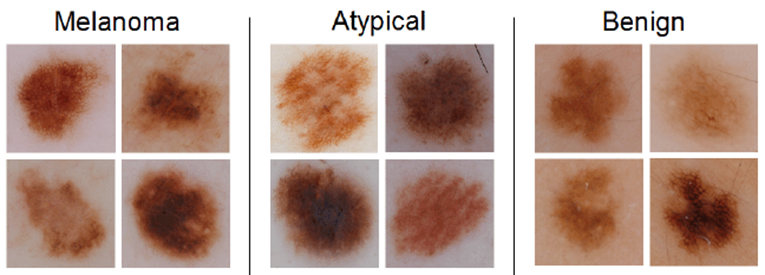
\includegraphics[scale = 0.5]{imagenes/Ejemplo2020.png}
	\caption{Ejemplo de imágenes de ISIC 2017}
	\label{fig:enter-label}
\end{figure}

\subsubsection{Uso de la galería de ISIC}

Como ya se mencionó anteriormente, el repositorio de ISIC contiene una galería donde encontrar imágenes y metadatos de diferentes enfermedades diagnosticadas por especialistas dermatólogos, y verificadas en gran cantidad de casos por biopsia. Este conjunto de datos, en la actualidad, puede ser más atractivo que la fusión de los  5 datasets descritos anteriormente, ya que desde el año 2020, no les ofrece ninguna mejora o procesado.

En total, podemos encontrar casi 80000 imágenes disponibles, siendo un total de 53781 imágenes correctamente etiquetadas y revisadas. Aunque se trata de unas 3500 imágenes menos que las competiciones en conjunto, la variedad de enfermedades e imágenes es mayor, ya que no se trata de las mismas imágenes empleadas en las competiciones, y no han sufrido ningún tipo de preprocesado o selección manual que pudiese alterar los resultados finales de forma positiva.

Por esta serie de argumentos, este conjuntos de imágenes será el empleado para realizar el diagnóstico de las enfermedades mediante la app móvil.

\subsection{ASAN Dataset}

ASAN \cite{Han2017,HAN20181529,HAN20189} es un conjunto de datos de origen surcoreano compuesto por lesiones malignas y benignas de la piel. Nos permiten obtener un mayor grado de variedad de las imágenes, ya que el repositorio ISIC se centra sobre todo en lesiones de piel de población europea y norteamericana.

\begin{table}[H]
	\centering
	\begin{tabular}{|c|c|}
		\hline
		\textbf{Tipo de lesión} & \textbf{Número de ejemplares} \\ \hline
		{Actinic keratoses and intraepithelial carcinoma (AKIEC)} & 651 \\ \hline
		{Basal Cell Carcinoma (BCC)} & 1082 \\ \hline
		{Dermatofibroma (DF)} & 1247 \\ \hline
		{Hereditary angioedema (HAO)} & 2715 \\ \hline
		{Intraepithelial Carcinoma (IC)} & 918 \\ \hline
		{Lentigo (LEN)} & 1193 \\ \hline
		{Melanoma (ML)} & 599 \\ \hline
		{Nevus (NV)} & 2706 \\ \hline
		{Pyogenic Granuloma (PG)}  & 375 \\ \hline
		{Squamous Cell Carcinoma (SCC)} & 1231 \\ \hline
		{Seborrhoeic Keratosis (SK)}  & 1423 \\ \hline
		{Wart} & 2985 \\ \hline
		\textbf{Total} & \textbf{17125} \\ \hline
	\end{tabular}
	\caption{Distribución de clases de ASAN dataset}
\end{table}

Tal y como se describe en la publicación de Goyal \cite{goyal2020artificial} , este dataset tiene 12 tipos de enfermedades, sumando un total de 17125 imágenes clínicas. Se dispone de escasa información acerca de este conjunto de datos, ya que los archivos de descarga no están acompañados por documentación acerca de su uso.


En las publicaciones asociadas a este conjunto de datos \cite{Han2017,HAN20181529,HAN20189}, se hace alusión a la existencia de varios subconjuntos de datos, designados de la A a la D, pero siendo el conjunto A el conjunto intersección de todos ellos. En la breve descripción de su publicación original \cite{Han2017}, podemos encontrar que existe un conjunto de imágenes de alta calidad sólo accesible bajo petición, y sólo se dispone de acceso público a sus miniaturas, las cuales se encuentran organizadas en grandes páginas de alta resolución en configuración de matriz. En caso de necesitar las imágenes por separado para entrenamiento, sería necesario separarlas manualmente.

Tampoco encontramos un fichero de metadatos donde se especifiquen atributos como la edad, la procedencia o el sexo del paciente, pero sí existe constancia de la verificación mediante biopsia de las imágenes gracias al nombre de las mismas, ya que cada matriz de imágenes tiene como nombre la clase a la que pertenecen, y si fue verificada o no por biopsia. Se requiere, por tanto, una fase de preprocesado inicial. El tamaño de cada miniatura es de 98 x 98, siendo un tamaño bastante reducido, en comparación con los 1024 x 1024 de las imágenes contenidas en ISIC.

Adicionalmente, podemos encontrar también 125 imágenes proporcionadas por el dataset Hallym, cuya procedencia es desconocida, pero que solo contiene imágenes cancerosas de tipo melanoma.

Teniendo en cuenta este segundo subconjunto, el dataset contiene un total de 12 clases:
\begin{itemize}
	\item Benignas: Dermatofibromas (acumulaciones de colágeno), Agiodemas hereditarios, lentigos (manchas debidas a exposición solar o por envejecimiento), nevus (lunares comunes de color marrón o azulado), granuloma piógeno (proliferación de capilares sanguíneos), queratósis seborreica (en forma de descamación de la piel) y verrugas comunes.
	 \item Malignas: Carcinomas intraepitelial, carcinoma de célula basal, melanomas (el más mortal e invasivo) y cáncer de células escamosas.
\end{itemize}

Encontramos, por tanto, una mayoría de imágenes benignas sobre malignas, lo cual puede introducir ciertos desequilibrios que provoquen sesgo a la hora del aprendizaje. Los resultados de la literatura con este dataset ronda el 90\% en el caso de que se empleen las imágenes de resolución completa. En \cite{HAN20189}, los resultados ofrecidos se acercan al 91\% de media, tras haber utilizado ResNet153 como arquitectura de red.


\begin{figure}[H]
	\centering
	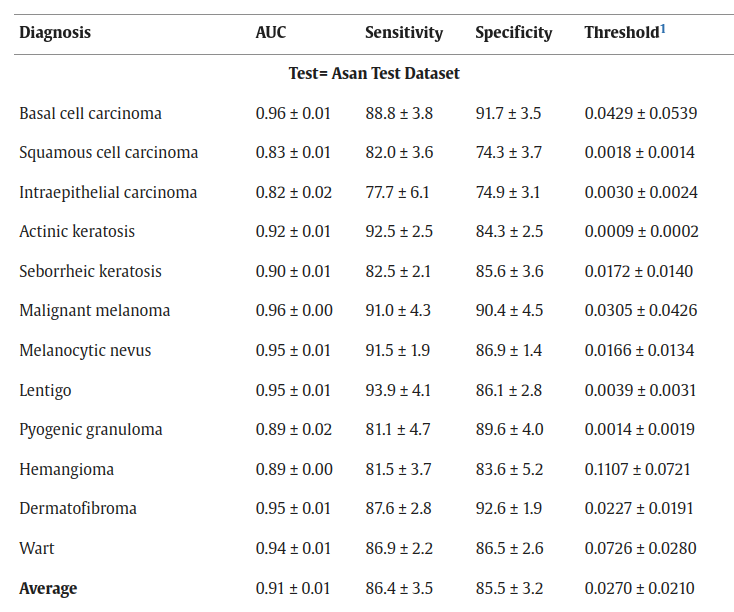
\includegraphics[scale = 0.4]{imagenes/results_asan.png}
	\caption{Ejemplo de lunares benignos en ASAN (Nevus)}
\end{figure}

Los resultados han sido confirmados por expertos dermatólogos y verificados en su mayoría mediante biopsia, por lo que las etiquetas asociadas a cada lesión están completamente verificadas. Como aspecto negativo, de cara al proyecto que se desarrolla en este documento, estos resultados distan bastante de lo que se puede conseguir con un smartphone, ya que, ResNet153 es uno de los modelos más profundos existentes en la literatura, y requieren grandes cantidades de memoria de gráficos. Además, sólo se dispone de las miniaturas, por lo que no será posible obtener características de grado fino aunque se aumente en profundidad o anchura el modelo. En preprocesado de datos, veremos algunas formas de evitar que se produzca esta penalización mediante la aplicación de mejora de imágenes con GANs.

\subsection{DermNet}

DermNet \cite{dermnetz} es un portal online que ofrece imágenes en alta resolución sobre lesiones cutáneas, tanto cancerígenas como benignas, para el uso como material docente para la formación de dermatólogos, y tiene a disposición un conjunto de imágenes complementado por datos en formato tabular, especialmente preparado para su uso en Inteligencia artificial.

Podemos encontrar enfermedades cutáneas recogidas de pacientes alrededor de todo el mundo, sin limitarse únicamente manchas  y lesiones parecidas a tumores cancerosos, y ofreciendo también heridas vinculadas a enfermedades infecciosas y hongos.  E incluso lesiones de tipo alérgico, así como acné, dermatitis severa o celulitis.

Estos datos se encuentran alojados de en una web que podemos visitar sin restricciones. Para facilitar la extracción,  existen gran cantidad de herramientas que podemos encontrar en GitHub \cite{githubdermnet}. En total, se pueden obtener hasta 23000 imágenes, compuestas por un total de 23 clases no balanceadas. Carecen de metadatos asociados, y además. poseen una marca de agua en la imagen que podría crear sesgos en el aprendizaje. Si se desea acceder a dicha información, es necesario solicitar permiso en su web oficial, y abonar una cantidad económica no especificada, determinada en función del  número de imágenes solicitadas y su procedencia.

Debido a la escasez de presupuesto, se descarta la opción de emplear este conjunto de datos, pero en la literatura podemos encontrar algunas menciones que datan del período anterior a 2020, momento en el cual parte de estos datos se ofrecía de forma abierta bajo otro portal de nombre similar, DermNet.


\subsection{ PH2}
El conjunto de datos PH2 \cite{ph2} es un conjunto de 200 imágenes obtenidas gracias al hospital Pedro Hispano de Portugal. Está compuesto por 200 imágenes de alta resolución que contienen 3 posibles casos de lesiones:
\begin{itemize}
	\item Lunar común (Common Nevus), 80 ejemplares
	\item Lunar atípico (Atypical Nevus), 80 ejemplares
	\item Melanomas, 40 ejemplares.
\end{itemize}

Dichas imágenes fueron captadas bajo las mismas condiciones, haciendo uso de un  sistema de análisis ``Tuebinger Mole Analyzer'', capaz de realkizar una magnificación de 20 veces mayor al tamaño original. Su resolución es de  768x560 pixeles, haciendo uso de los 3 habituales canales RGB a 8 bit de profundidad cada uno. Se trata de unas imágenes de buena calidad, que llevan su correspondiente información asociada en forma de metadatos. Estos describen el color, la extensión de las manchas, la textura, la forma del borde, la localización, y otro tipo de características, como el tipo de piel.

De acuerdo a los requisitos especificados en su web, \cite{ph2data}, podemos acceder a los datos  y sus metadatos asociados de forma totalmente abierta y sin restricciones siempre que su uso se limite fines académicos y personales, como es este caso.
\begin{figure}[H]
	\centering
	\label {ph2}
	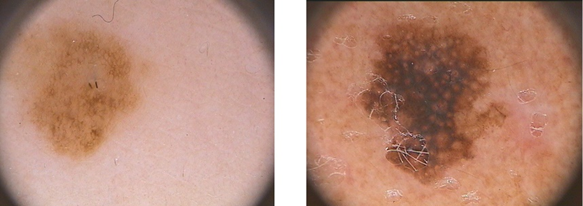
\includegraphics[scale = 0.6]{imagenes/PH2.png}
	\caption{Nevus maligno y benigno en PH2}
\end{figure}

En la figura \ref{ph2} podemos encontrar una muestra de estas imágenes, concretamente un lunar común (nevus) y un lunar de tipo cancerígeno.

\subsection{PAD-UFES 20}
A patient may have one or more skin lesions and a skin lesion may have one or more images. In total, there are 1373 patients, 1641 skin lesions, and 2298 images present in the dataset. 
PAD-UFES-20 \cite{PACHECO2020106221} se trata de un conjunto de imágenes disponible públicamente acerca de lesiones cutáneas benignas y malignas. Concretamente, dispone de imágenesde 1.641 lesiones cutáneas únicas recopiladas, procedenetes de 1373 pacientes. Tal y como se especifica en su publicación \cite{PACHECO2020106221}, cada paciente perteneciente al dataset puede ofrecer imágenes de piel sana, una lesión, o varias de ellas. Por tanto, el conteo final de imágenes asciende a un total de 2.298 ejemplares.

Las imágenes a analizar han sido extraídas en sus totalidad de dispositivos móviles, los cuales se conectaban a un servidor al cual enviaban la imagen para su posterior diagnóstico y validación mediante biopsia en caso de sospecha de caso positivo de cáncer. Todas ellas fueron almacenadas de forma directa, sin aplicar ningún tipo de ecualización o filtro, ya que el formato de guardado escogido es PNG, caracterizado por ser un formato sin pérdidas.

Entre sus clases, podemos encontrar, de forma equilibrada tres enfermedades benignas de la piel y tres tipos de cánceres de piel:

\begin{itemize}
	\item Queratosis actínica: manchas escamosas y oscurecidas en la piel debido a la exposición solar. Benignas de naturaleza.
	\item Cáncer de células basales: tumores generalmente aislados que surgen en las capas profundas de la piel
	\item Melanoma: tumores y manchas cancerosas de color oscuro, en algunos casos acompañadas de necrosis de tejidos, y altamente mortal
	\item Nevus: lunares comunes
	\item Queratosis seborreica: enfermedad benigna, que forma manchas protuberantes de color oscuro no contagiosas.
	\item Cáncel de células escamosas: cancer con baja tasa de mortalidad, que surge en la capa intermedia de la piel, y cuyo crecimiento puede tener graves riesgos para la salid.
	\end{itemize}

 Todos estos datos fueron revisados por dermatólogos expertos, quie aportaron metadatos muy detallados acerca del historial del paciente, gracias a la asociación con la Unidad Patológica de Anatomía del Hospital universitario Cassiano Antonio Moraes (HUCAM) , perteneciente a la Universidad Federal de Espírito Santo, en Brasil. EDe entre los metadatos ofrecidos, podemos destacar:

\begin{itemize}
	\item ID de paciente
	\item ID de lesión,
	\item ID de imagen
	\item Si la lesión benigna fue o no probada por biopsia.
	\item Enfermedad diagnosticada
	\item Información del paciente: fumador o no, localización de la lesión, edad, exposición a químicos, historial cancerígeno, etc.
\end{itemize}

En su publicación original\cite{PACHECO2020106221}, podemos encontrar un resumen de su contenido de forma más específica:

\begin{table}[!ht]
	\centering
	\begin{tabular}{|c|c|c|}
		\hline
		\textbf{Diagnóstico} & \textbf{Ejemplares} & \textbf{\% biopsied} \\ \hline
		Actinic Keratosis (ACK) & 730 & 24.4\% \\ \hline
		Basal Cell Carcinoma of skin (BCC) & 845 & 100\% \\ \hline
		Malignant Melanoma (MEL) & 52 & 100\% \\ \hline
		Melanocytic Nevus of Skin (NEV) & 244 & 24.6\% \\ \hline
		Squamous Cell Carcinoma (SCC) & 192 & 100\% \\ \hline
		Seborrheic Keratosis (SEK)	&235	&6.4 \% \\ \hline
		\textbf{Total} & \textbf{2298} & \textbf{58.4\%} \\ \hline
	\end{tabular}
	\caption{Tabla de casos diagnosticados en PAD-UFES20}
\end{table}

Donde podemos apreciar que todos los casos de enfermedades cancerígenas han sido probados mediante biopsia, y el cáncer de célula basal se trata del tipo de enfermedad más frecuente.
\begin{figure}[H]
	\centering
	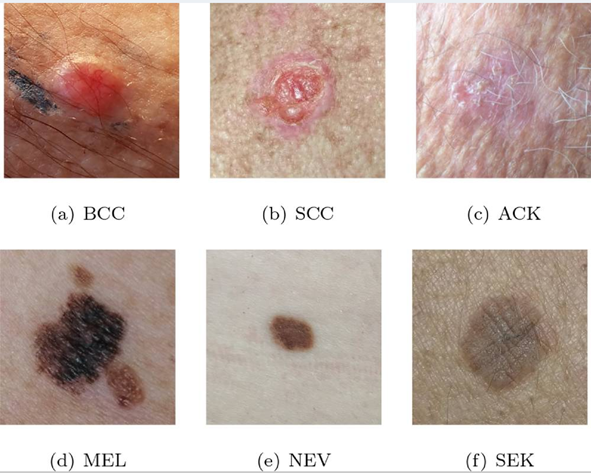
\includegraphics[scale = 0.5]{imagenes/PAD-UFES.png}
	\caption{Batch de ejemplo de PAD-UFES 20 \cite{PACHECO2020106221}}
\end{figure}

La gran ventaja de este dataset es que sus imágenes han sido recopiladas mediante smartphones, por lo que las condiciones de recopilación han sido prácticamente idénticas a las que se recibirán por el modelo entrenado para este trabajo. Esto nos aporta como beneficio un conjunto de entrenamiento mucho más cercano a la población real a la que será destinada el modelo.

\subsection{Severance}

Severance es otro conjunto de lesiones cutáneas que podemos encontrar para su libre acceso de forma digital \cite{severance}. Se trata de un conjunto de imágenes de lesiones cutáneas recopiladas de pacientes de Corea del Sur por el hospital Severance.  Los datos recopilados pertenecen a los casos diagnosticados por dermatólogos entre enero de 2008 y marzo de 2019, teniendo en cuenta el historial medido de cada uno de los pacientes y asegurando un grado alto de confianza en el diagnóstico.

La población de este muestreo se centra sobre pacientes mayores a 19 años, que fueron diagnosticados con lesiones provenientes de tumores. Se excluyó de este estudio a todas aquellas lesiones de difícil acceso, como las lesiones intraoculares, postoperatorias, o causas por medios externos, como láseres o costuras operatorias. Además, algunos pacientes tenían diferentes lesiones en zonas próximas, por lo que se tomaron las imágenes de forma que el diagnóstico para cada una de ellas fuera individual, y no se pudieran producir incongruencias entre los expertos en el diagnóstico. 

En total, se dispone de 40331 imágenes clínicas, que provienen de 10426 pacientes distintos que participaron en la cesión de datos. Al igual que ASAN, este dataset posee distintas versiones publicadas en la red, siendo accesible únicamente su partición A, y podemos encontrar 38 tipos de diagnósticos distintos de los 43 disponibles en total,  los cuales no siguen una distribución equilibrada.

Realizando un test estadístico previo, es posible verificar que las 6 clases más comunes contenidas en este dataset componen el 75\% del conjunto total. Está compuesto por queratosis actínica (22.5\%), angiofibromas (14.4\%), angiokeratomas(13.8\%), cáncer células basales (8.1\%), lunares de Becker (7.5\%), bluenevus (6.2\%), y la enfermedad de Bowen (carcinomas)(6.1\%).

El interés en este dataset se debe a que algunas de estas clases mayoritarias, como los nevus azules y los lunares de Becker, son condiciones benignas que suelen ser retirados únicamente con fines estéticos, permitiendo complementar con el resto de los diagnósticos negativos. Este tipo de lunares son los más complejos de diagnosticar, debido a sus colores similares a un melanoma, y suelen requerir una biopsia, por lo que su diagnóstico suele alargarse.

Las imágenes publicadas son miniaturas recogidas en forma de matriz, presentando un formato similar a las encontradas en ASAN. La diferencia, en este caso, es que disponemos de los metadatos asociados a cada imagen, y el proceso de separación de miniaturas se ve simplificado. En la figura \ref{fig:sevimg} podemos apreciar el formato matricial, y la toma de imágenes desde diferentes puntos de vista para portar una mayor variabilidad al modelo. Es posible separar cada una de estas imágenes logrando un conjunto de aproximadamente 10400 fotografías a 98 x 98 píxeles en formato jpeg, debido a la compresión con pérdidas aplicada para almacenarlas.

\begin{figure}[H]
	\centering
	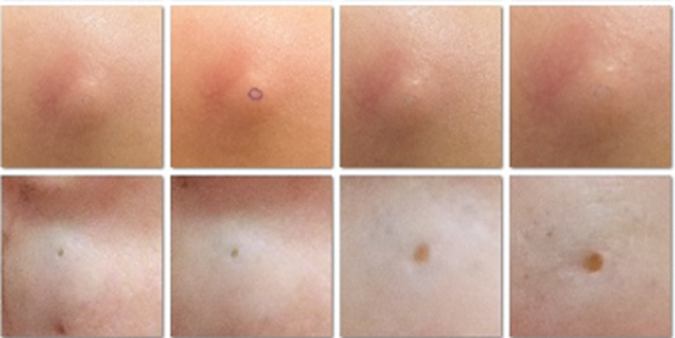
\includegraphics[scale = 0.5]{imagenes/Severance.png}
	\caption{Imágenes de ejemplo provenientes del dataset Severance   }
	 \label{fig:sevimg}
\end{figure}

En cuanto a los resultados obtenidos en tareas de aprendizaje, de nuevo encontramos que se han utilizado grandes modelos para realizar el aprendizaje, siendo en este caso utilizado los modelos VGG16 y ResNext50, y siendo el resultado de accuracy top1 un 53.0\%,  dada a la complejidad del problema al utilizar clases infrarepresentadas.

\subsection{Otros datasets}

En los puntos anteriores, se han descritos los datasets disponibles con mayores referencias y mayor peso dentro del espacio de investigación cubierto por el campo de investigación acerca del cáncer de piel. Pero, existe una serie de bases de datos con grandes cantidades de datos que fueron retiradas de su acceso público, o simplemente, fueron eliminadas debido a limitaciones legales por licencias. A continuación, se destacan algunas de ellas que tuvieron un gran impacto en la literatura de los años 2015 y 2020:

\begin{itemize}
	\item \textbf{DermQuest}. Se trataba de un atlas virtual que contenía información detallada acerca de lesiones cutáneas, con el fin de servir como atlas de estudio para dermatólogos en formación. Esta información, a pesar de ser principamente académica, podía ser recopilada por técnicas de minería de datos.  Posteriormente, este conjunto de datos fue dado de baja, pero reapareció como un subconjunto del repositorio Derm101. Sin embargo, desapareció de forma definitiva en el año 2019, por lo que no es posible encontrar estos datos para uso.
	
	\item \textbf{SD-198 y SD-260}  \cite{10.1007/978-3-319-46466-4_13} son dos datasets de origen chino que recopilan fotografías y metadatos acerca de  98 y 260 imágenes respectivamente, asegurándo al menos un total de 50 imágenes como mínimo por patología. Ambos datasets se pueden ver referenciados en mutitud de papers como \cite{goyal2020artificial}. Habitualmente, el más usado de ambas variantes era SD-198. Existen datasets con mayor y menor cantidad de clases, pero son subconjuntos de estos, ya que los datasets se organizaban en niveles de carpetas, donde cada nivel descendido aportaba un mayor nivel de granularidad en el diagnóstico. En la actualidad, sólo el subconjunto 198 permanece en línea, pero bajo solicitud. Contiene 6,584 imágenes, que fueron capturadas para historias clínicas mediante smartphones. Sin embargo, debido a las dificultades del idioma, y la dificultad de contacto con el autor original, se prescindirá de este dataset para el estudio del problema.
	\item \textbf{DermIS} \cite {dermis} es un atlas online creado con fines académicos. Aunque no dispone de metainformación asociada, podría emplearse para el  problema que se trata en este trabajo. Pero, debido a la incorporación de otras enfermedades que no vinculan con el dominio del problema, se descarta su utilización.
	\item \textbf{Mednode} \cite{GIOTIS20156578} contiene 70 melanomas and 100 nevus provenientes del  Departamento de dermatologia de la universidad University Medical Center Groningen (UMCG) , cuyo objetivo es la creación de una aplicación de diagnóstico de enfermedades cutáneas no desmocópicas que faciliten la decisión a los dermatólogos. Debido a su pequeño tamaño, y a que este aporta datos acerca de clases ya mayoritarias en otros datasets, se propone su no utilización para el experimento.
\end{itemize}

Además de estos datasets no disponibles en la actualidad, existen publicaciones recientes sobre nuevos conjuntos de datos utilizados de uso interno para dicha investigación, fortaleciendo así la visión de que la inteligencia artificial aplicada a la dermatología es un campo de interés y competitividad. No es posible acceder a este tipo de conjuntos debido a su gran valor competitivo dentro de la industria  de las aplicaciones de asistencia al diagnóstico dermatológico.